%% Relatorio Tecnico - Desafio 1: Sistema de Contagem de Parafusos
%% Bootcamp CDIA - Programa de Residencia em IA
\documentclass[12pt,a4paper]{article}

%% --- Pacotes ---
\usepackage[utf8]{inputenc}
\usepackage[T1]{fontenc}
\usepackage[brazil]{babel}
\usepackage{geometry}
\usepackage{graphicx}
\usepackage{amsmath}
\usepackage{amssymb}
\usepackage{booktabs}
\usepackage{longtable}
\usepackage{array}
\usepackage{xcolor}
\usepackage{listings}
\usepackage{hyperref}
\usepackage{float}
\usepackage{caption}
\usepackage{subcaption}
\usepackage{enumitem}
\usepackage{fancyhdr}
\usepackage{titlesec}
\usepackage{parskip}
\usepackage[stretch=0]{microtype}  %% desativa expansao de fonte (incompativel com fontes bitmap)
\usepackage{setspace}
\setlength{\headheight}{14pt}  %% corrige aviso do fancyhdr
\usepackage{colortbl}
\usepackage{mdframed}
\usepackage{tcolorbox}
\tcbuselibrary{skins,breakable}

%% --- Geometria da pagina ---
\geometry{top=2.5cm, bottom=2.5cm, left=3cm, right=2.5cm}

%% --- Cores ---
\definecolor{codebg}{RGB}{245,245,245}
\definecolor{codeframe}{RGB}{180,180,180}
\definecolor{primary}{RGB}{0,70,140}
\definecolor{accent}{RGB}{20,130,255}
\definecolor{darkgray}{RGB}{60,60,60}
\definecolor{green}{RGB}{20,120,60}
\definecolor{amber}{RGB}{180,100,0}
\definecolor{red}{RGB}{160,20,20}
\definecolor{lightblue}{RGB}{230,240,255}
\definecolor{lightgreen}{RGB}{230,250,235}
\definecolor{lightyellow}{RGB}{255,252,230}

%% --- Caixas coloridas ---
\tcbset{
  veredicto/.style={
    colback=lightblue, colframe=primary,
    fonttitle=\bfseries, title=#1,
    breakable, arc=4pt
  },
  vantagem/.style={
    colback=lightgreen, colframe=green,
    fonttitle=\bfseries\color{green}, title=#1,
    arc=4pt
  },
  limitacao/.style={
    colback=lightyellow, colframe=amber,
    fonttitle=\bfseries\color{amber}, title=#1,
    arc=4pt
  },
}

%% --- Configuracao de listagens de codigo ---
\lstset{
  backgroundcolor=\color{codebg},
  basicstyle=\ttfamily\footnotesize,
  breaklines=true,
  captionpos=b,
  commentstyle=\color{gray}\itshape,
  frame=single,
  framerule=0.5pt,
  rulecolor=\color{codeframe},
  keepspaces=true,
  keywordstyle=\bfseries\color{primary},
  language=Python,
  morekeywords={Path,YOLO,FastAPI,Session,Depends,UploadFile,Form,File,Request,dataclass},
  numbers=left,
  numbersep=6pt,
  numberstyle=\tiny\color{gray},
  showspaces=false,
  showstringspaces=false,
  tabsize=4,
  xleftmargin=14pt,
  stringstyle=\color{accent},
}

%% --- Cabecalho e rodape ---
\pagestyle{fancy}
\fancyhf{}
\fancyhead[L]{\small\color{darkgray}Sistema de Contagem de Parafusos -- Desafio 1}
\fancyhead[R]{\small\color{darkgray}Bootcamp CDIA}
\fancyfoot[C]{\small\thepage}
\renewcommand{\headrulewidth}{0.4pt}

%% --- Titulos de secao com cor ---
\titleformat{\section}{\large\bfseries\color{primary}}{}{0em}{\thesection\quad}
\titleformat{\subsection}{\normalsize\bfseries\color{darkgray}}{}{0em}{\thesubsection\quad}
\titleformat{\subsubsection}{\normalsize\itshape\color{darkgray}}{}{0em}{\thesubsubsection\quad}

%% --- Hiperlinks ---
\hypersetup{colorlinks=true, linkcolor=primary, urlcolor=accent, citecolor=primary}

%% ============================================================
\begin{document}

%% ============================================================
%% CAPA
%% ============================================================
\begin{titlepage}
  \centering
  \vspace*{1.8cm}
  {\huge\bfseries\color{primary}
    Sistema Inteligente de Contagem\\[0.4em]
    de Parafusos para Picking Industrial\\[1.2em]}
  {\large\color{darkgray}
    Relat\'orio T\'ecnico -- Desafio 1\\
    Bootcamp de Ci\^encia de Dados e Intelig\^encia Artificial (CDIA)\\
    Programa de Resid\^encia em IA\\[1.8cm]}
  \rule{\linewidth}{0.5pt}\\[0.4em]
  {\normalsize
    \textbf{Autor:} Ana Rafaely\\[0.3em]
    \textbf{Data:} 30 de maio de 2026\\[0.3em]
  }
  \rule{\linewidth}{0.5pt}\\[1.2cm]
  \begin{tcolorbox}[colback=lightblue, colframe=primary, arc=6pt,
                    title={\bfseries Solu\c{c}\~oes desenvolvidas e comparadas \quad(vers\~ao 2)}]
    \begin{tabular}{ll}
      \textbf{Solu\c{c}\~ao 1} & Vis\~ao Cl\'assica com OpenCV\\
                                & (pipeline de segmenta\c{c}\~ao adaptativa)\\[4pt]
      \textbf{Solu\c{c}\~ao 2} & Aprendizado Profundo com YOLOv11\\
                                & (detec\c{c}\~ao supervisionada) -- \emph{recomendada}\\[4pt]
      \textbf{Evolu\c{c}\~ao}  & Modelo Fundacional SAM3\\
                                & (futuro escal\'avel, requer GPU dedicada)\\
    \end{tabular}
  \end{tcolorbox}
  \vfill
  {\small\color{gray}
    Tecnologias: Python 3 $\cdot$ OpenCV $\cdot$ YOLOv11 (Ultralytics) $\cdot$
    FastAPI $\cdot$ SQLite $\cdot$ Jinja2 $\cdot$ scikit-learn (DBSCAN)
  }
\end{titlepage}

%% --- Sumario -------
\tableofcontents
\newpage

%% ============================================================
\section{Introdu\c{c}\~ao e Contexto do Problema}

Uma empresa metal-mec\^anica solicitou ao Programa de Resid\^encia em IA o desenvolvimento de
um sistema capaz de automatizar a contagem de parafusos no processo de \emph{picking}: a
coleta e embalagem de itens que ser\~ao enviados a clientes. Atualmente, a contagem \'e
realizada manualmente por funcion\'arios que registram a quantidade em um \emph{smartphone}
corporativo, processo suscet\'ivel a erros humanos decorrentes de fadiga e alto volume de
pedidos.

\subsection{Objetivos}

\begin{enumerate}[leftmargin=*, label=\arabic*.]
  \item Desenvolver um sistema de vis\~ao computacional capaz de contar parafusos em
        fotografias tiradas por smartphones.
  \item Implementar a solu\c{c}\~ao em Python.
  \item Preparar relat\'orio t\'ecnico com metodologia, modelos e resultados.
\end{enumerate}

\subsection{Restri\c{c}\~oes}

\begin{itemize}[leftmargin=*]
  \item A solu\c{c}\~ao deve operar nos smartphones j\'a dispon\'iveis (baixo recurso
        computacional).
  \item A interface deve ser simples para operadores sem treinamento t\'ecnico.
  \item Apenas \textbf{5 imagens} foram fornecidas inicialmente, exigindo criatividade
        na aquisi\c{c}\~ao ou augmenta\c{c}\~ao de dados.
\end{itemize}

\subsection{Estrat\'egia adotada}

Diante da complexidade do problema e das restri\c{c}\~oes, foram desenvolvidas
\textbf{duas solu\c{c}\~oes independentes} e uma \textbf{aplica\c{c}\~ao web compartilhada},
permitindo compara\c{c}\~ao direta de abordagens:

\begin{itemize}[leftmargin=*]
  \item \textbf{Solu\c{c}\~ao 1:} pipeline cl\'assico de vis\~ao computacional com OpenCV --
        sem treinamento, interpret\'avel, leve.
  \item \textbf{Solu\c{c}\~ao 2:} detec\c{c}\~ao supervisionada com YOLOv11 -- treinada
        em dataset p\'ublico anotado, robusta e precisa.
\end{itemize}

\subsection{Perspectiva de Evolu\c{c}\~ao Futura -- Modelos Fundacionais (SAM3)}
\label{sec:sam3}

Al\'em das duas solu\c{c}\~oes implementadas, registra-se desde j\'a uma \textbf{terceira
via, considerada para a escalabilidade futura}: o uso de \emph{modelos fundacionais de
segmenta\c{c}\~ao}, em especial o \textbf{SAM3} (\emph{Segment Anything Model}, da
Meta AI) -- um modelo do tipo LLM/\emph{foundation model} aplicado \`a vis\~ao
computacional, capaz de segmentar praticamente qualquer objeto em uma imagem com pouco
ou nenhum treinamento espec\'ifico (\emph{zero-shot} / \emph{few-shot}).

\begin{tcolorbox}[veredicto={Por que o SAM3 N\~AO foi adotado neste projeto}]
\textbf{Decis\~ao:} o SAM3 \emph{n\~ao} \'e aplic\'avel ao cen\'ario atual da empresa,
em raz\~ao das \textbf{restri\c{c}\~oes de recurso computacional}.

\medskip
Modelos fundacionais como o SAM3 possuem centenas de milh\~oes a bilh\~oes de
par\^ametros, exigindo \textbf{GPU dedicada com alta mem\'oria} para infer\^encia em
tempo h\'abil. Isso \'e \textbf{incompat\'ivel} com o requisito central do desafio:
execu\c{c}\~ao nos \emph{smartphones de baixo custo} j\'a dispon\'iveis no time de
\emph{picking}.

\medskip
\textbf{Quando o SAM3 seria uma op\c{c}\~ao vi\'avel:} caso a empresa venha a investir
em infraestrutura -- por exemplo, um \textbf{servidor central com GPU} que processasse
as imagens enviadas pelos smartphones via rede -- o SAM3 se tornaria uma alternativa
poderosa, pois:
\begin{itemize}[leftmargin=*, noitemsep]
  \item eliminaria a necessidade de anotar e treinar datasets espec\'ificos;
  \item generalizaria imediatamente para novos tipos de pe\c{c}as (porcas, arruelas,
        pinos) sem re-treinamento;
  \item permitiria segmenta\c{c}\~ao em n\'ivel de \emph{pixel}, melhorando a contagem
        em aglomerados densos e com sobreposi\c{c}\~ao severa.
\end{itemize}

\medskip
\textbf{Conclus\~ao:} o SAM3 fica registrado como \textbf{caminho de evolu\c{c}\~ao
escal\'avel} para um cen\'ario futuro com maior or\c{c}amento de infraestrutura,
enquanto as Solu\c{c}\~oes 1 e 2 atendem o requisito atual de baixo custo.
\end{tcolorbox}

Portanto, abaixo destacaremos as soluções aplicadas nesse projeto, com detalhes técnicos, resultados práticos e análises comparativas.

%% ============================================================
\section{Solu\c{c}\~ao 1 -- Vis\~ao Cl\'assica com OpenCV}
\label{sec:sol1}

\subsection{Motiva\c{c}\~ao}

Uma abordagem cl\'assica foi escolhida como \emph{baseline} por ser:
\begin{itemize}[leftmargin=*]
  \item \textbf{Zero-shot:} n\~ao requer dados anotados nem treinamento.
  \item \textbf{Interpret\'avel:} cada etapa pode ser inspecionada visualmente.
  \item \textbf{Extremamente leve:} roda em qualquer dispositivo com OpenCV.
  \item \textbf{R\'apida de implantar:} basta instalar as depend\^encias e executar.
\end{itemize}

\subsection{Arquitetura do Pipeline}

O m\'odulo central \'e \texttt{screw\_counter.py}, com mais de 1.000 linhas que implementam
um pipeline modular em quatro camadas:

\begin{center}
\fbox{
\begin{minipage}{0.88\textwidth}
\centering
\textbf{Camada 1: An\'alise da Cena} (\texttt{classify\_scene})\\
$\downarrow$\\
\textbf{Camada 2: Segmenta\c{c}\~ao adaptativa} (\texttt{segment\_image} -- 6 modos)\\
$\downarrow$\\
\textbf{Camada 3: Detectores paralelos} (contornos + watershed + DBSCAN)\\
$\downarrow$\\
\textbf{Camada 4: Ensemble e sele\c{c}\~ao} (\texttt{\_choose\_ensemble})
\end{minipage}
}
\end{center}

\subsubsection{Camada 1 -- An\'alise de Cena}

Antes de qualquer segmenta\c{c}\~ao, a fun\c{c}\~ao \texttt{classify\_scene} calcula
indicadores visuais que caracterizam a cena e recomendam o modo mais adequado:

\begin{lstlisting}[caption={An\'alise de cena para escolha autom\'atica de modo}]
def classify_scene(img_bgr: np.ndarray) -> dict[str, Any]:
    gray = cv2.cvtColor(img_bgr, cv2.COLOR_BGR2GRAY)
    mean_brightness  = float(np.mean(gray))
    contrast         = float(np.std(gray))
    light_bg_ratio   = float(np.mean(gray > 185))

    lap = cv2.Laplacian(gray, cv2.CV_32F)
    noise_estimate  = float(np.std(lap))
    texture_ratio   = float(np.mean(np.abs(lap) > max(12.0, noise_estimate * 0.45)))

    # Calcula densidade e toque entre objetos
    if touching_score > 0.25 or density > 0.15:
        mode = "modo_denso"
    elif scale_variation > 3.0:
        mode = "modo_multiescala"
    elif tray_like:
        mode = "modo_bandeja"
    elif textured:
        mode = "modo_texturizado"
    elif light_bg_ratio > 0.55:
        mode = "modo_claro"
    else:
        mode = "modo_cinza"
    return {..., "recommended_mode": mode}
\end{lstlisting}

\subsubsection{Camada 2 -- Segmenta\c{c}\~ao Adaptativa (6 Modos)}

Cada modo usa uma combina\c{c}\~ao espec\'ifica de filtros e limiares. A
Tabela~\ref{tab:modos} resume as estrat\'egias.

\begin{table}[H]
  \centering
  \caption{Modos de segmenta\c{c}\~ao e suas estrat\'egias}
  \label{tab:modos}
  \begin{tabular}{lp{9cm}}
    \toprule
    \textbf{Modo} & \textbf{Estrat\'egia principal} \\
    \midrule
    \texttt{modo\_claro}       & Otsu invertido + Canny; fundo branco/claro \\
    \texttt{modo\_cinza}       & Gradiente morfol\'ogico + Otsu; fundo cinza \\
    \texttt{modo\_bandeja}     & CLAHE no canal L* (LAB) + gradiente; fundos coloridos \\
    \texttt{modo\_texturizado} & Top-hat para remover fundo + gradiente; fundos com textura \\
    \texttt{modo\_denso}       & Bilateral + limiar adaptativo + Otsu combinados; objetos agrupados \\
    \texttt{modo\_multiescala} & Gradiente em tr\^es escalas (0.75$\times$, 1.0$\times$, 1.25$\times$) \\
    \bottomrule
  \end{tabular}
\end{table}

\subsubsection{Camada 3 -- Detectores}

Tr\^es detectores s\~ao aplicados em paralelo sobre a mesma m\'ascara:

\begin{description}[leftmargin=*, style=nextline]
  \item[\texttt{detector\_contours}:] extrai componentes conectados e estima
    multiplicidade por raz\~ao de \'area ($\text{mult} = \lfloor A_c / A_{\text{ref}} \rceil$
    quando $A_c > 1.75 \cdot A_{\text{ref}}$).

  \item[\texttt{detector\_watershed}:] aplica \emph{distance transform} e localiza picos
    (m\'aximos locais) para separar parafusos sobrepostos.

  \item[\texttt{detector\_fragmentos\_dbscan}:] agrupa fragmentos pequenos por DBSCAN
    (quando muitos componentes s\~ao menores que $0.7 \cdot A_{\text{ref}}$), contando
    cada \emph{cluster} como um parafuso.
\end{description}

\begin{lstlisting}[caption={Watershed: picos do distance transform como separadores}]
def _distance_peaks(mask, ref_area, min_distance=None):
    dist = cv2.distanceTransform(mask_bin, cv2.DIST_L2, 5)
    if min_distance is None:
        min_distance = max(int(np.sqrt(ref_area / np.pi) * 0.62), 5)
    smooth = cv2.GaussianBlur(dist, (0, 0), sigmaX=min_distance / 2.5)
    dilated = cv2.dilate(smooth, _kernel(2 * min_distance + 1))
    peak_mask[(smooth == dilated) & (smooth > smooth.max() * 0.28)] = 255
    n_peaks, _, _, _ = cv2.connectedComponentsWithStats(peak_mask, 8)
    return dist, peak_mask, n_peaks - 1
\end{lstlisting}

\subsubsection{Camada 4 -- Ensemble e Sele\c{c}\~ao}

Com o modo \texttt{ensemble=True}, a fun\c{c}\~ao \texttt{\_choose\_ensemble}
combina os resultados de todos os modos e detectores (at\'e $6 \times 3 + 1 = 19$
candidatos), selecionando o mais estable por um score ponderado:

$$\text{score} = 1.2 \cdot \overline{\text{conf}} + \frac{1}{1 + |c - \text{mediana}|} - 0.05 \cdot \text{rank}$$

onde $\overline{\text{conf}}$ \'e a confian\c{c}a m\'edia das detec\c{c}\~oes e
$\text{rank}$ penaliza detectores menos adequados para a cena atual.

\subsection{Estima\c{c}\~ao de \'Area de Refer\^encia}

A \'area de um parafuso individual (\texttt{ref\_area}) \'e estimada automaticamente:

\begin{lstlisting}[caption={Estima\c{c}\~ao robusta da \'area de refer\^encia}]
def estimate_ref_area(components, fallback=4021.0):
    areas = sorted(float(c.area) for c in components)
    if len(areas) >= 4:
        # Remove 20% dos extremos (outliers) antes da mediana
        trimmed = areas[int(len(areas)*0.20) : int(len(areas)*0.80)]
        ref = float(np.median(trimmed or areas))
    else:
        ref = float(np.median(areas))
    return float(np.clip(ref, fallback * 0.45, fallback * 2.5))
\end{lstlisting}

\subsection{Modulo de Calibra\c{c}\~ao}

A fun\c{c}\~ao \texttt{calibrate\_from\_single\_screw} permite que o operador fotografe
um \'unico parafuso centralizado para calibrar a \texttt{ref\_area} antes do uso.
O sistema retorna confian\c{c}a (\emph{alta/m\'edia/baixa}) e orienta\c{c}\~oes ao usu\'ario.

\subsection{Avalia\c{c}\~ao e M\'etricas}

O m\'odulo \texttt{metrics.py} define as m\'etricas de avalia\c{c}\~ao:
\textbf{MAE} (erro absoluto m\'edio), \textbf{acur\'acia exata}, \textbf{vi\'es m\'edio},
supercontagens e subcontagens. O script \texttt{evaluation.py} executa avalia\c{c}\~ao
em lote, salva grades de debug e gera relat\'orio Markdown autom\'atico.

\begin{lstlisting}[caption={M\'etricas de avalia\c{c}\~ao (\texttt{metrics.py})}]
def mean_absolute_error(y_true, y_pred):
    """Media dos erros absolutos (MAE)."""
    return float(np.mean(np.abs(np.asarray(y_true) - np.asarray(y_pred))))

def exact_match_accuracy(y_true, y_pred):
    """Proporcao de contagens exatamente corretas."""
    return float(np.mean(np.asarray(y_true) == np.asarray(y_pred)))

def mean_bias_error(y_true, y_pred):
    """Vies medio: positivo = supercontagem, negativo = subcontagem."""
    return float(np.mean(np.asarray(y_pred) - np.asarray(y_true)))
\end{lstlisting}

\subsection{Qualidade de Captura}

A fun\c{c}\~ao \texttt{\_estimate\_capture\_quality} analisa a imagem e emite alertas
ao operador: foto tremida (score de Laplaciano), objetos muito pequenos (dist\^ancia),
parafusos cortados na borda, e baixa confian\c{c}a do ensemble.

\begin{tcolorbox}[limitacao={Limita\c{c}\~oes da Solu\c{c}\~ao 1}]
\begin{itemize}[leftmargin=*, noitemsep]
  \item Sens\'ivel a varia\c{c}\~oes de ilumina\c{c}\~ao e fundo.
  \item Parafusos fortemente sobrepostos podem ser contados como um \'unico blob.
  \item Fundos muito texturizados confundem o segmentador.
  \item N\~ao generaliza para novos tipos de parafusos sem reajuste de par\^ametros.
\end{itemize}
\end{tcolorbox}

%% --- Resultados Praticos OpenCV ---
\subsection{Resultados Pr\'aticos -- Testes com Novas Imagens}

Para validar o pipeline cl\'assico em condi\c{c}\~oes reais, o sistema foi testado com
novas imagens fornecidas fora do conjunto de calibra\c{c}\~ao. A
Figura~\ref{fig:opencv-resultados} apresenta tr\^es resultados representativos, onde
cada parafuso detectado recebe uma caixa delimitadora colorida de acordo com o detector
que o identificou (\textcolor{green}{verde} = contorno isolado,
\textcolor{orange}{laranja} = watershed, \textcolor{red}{vermelho} = DBSCAN).

\begin{figure}[H]
  \centering
  \begin{subfigure}[t]{0.31\textwidth}
    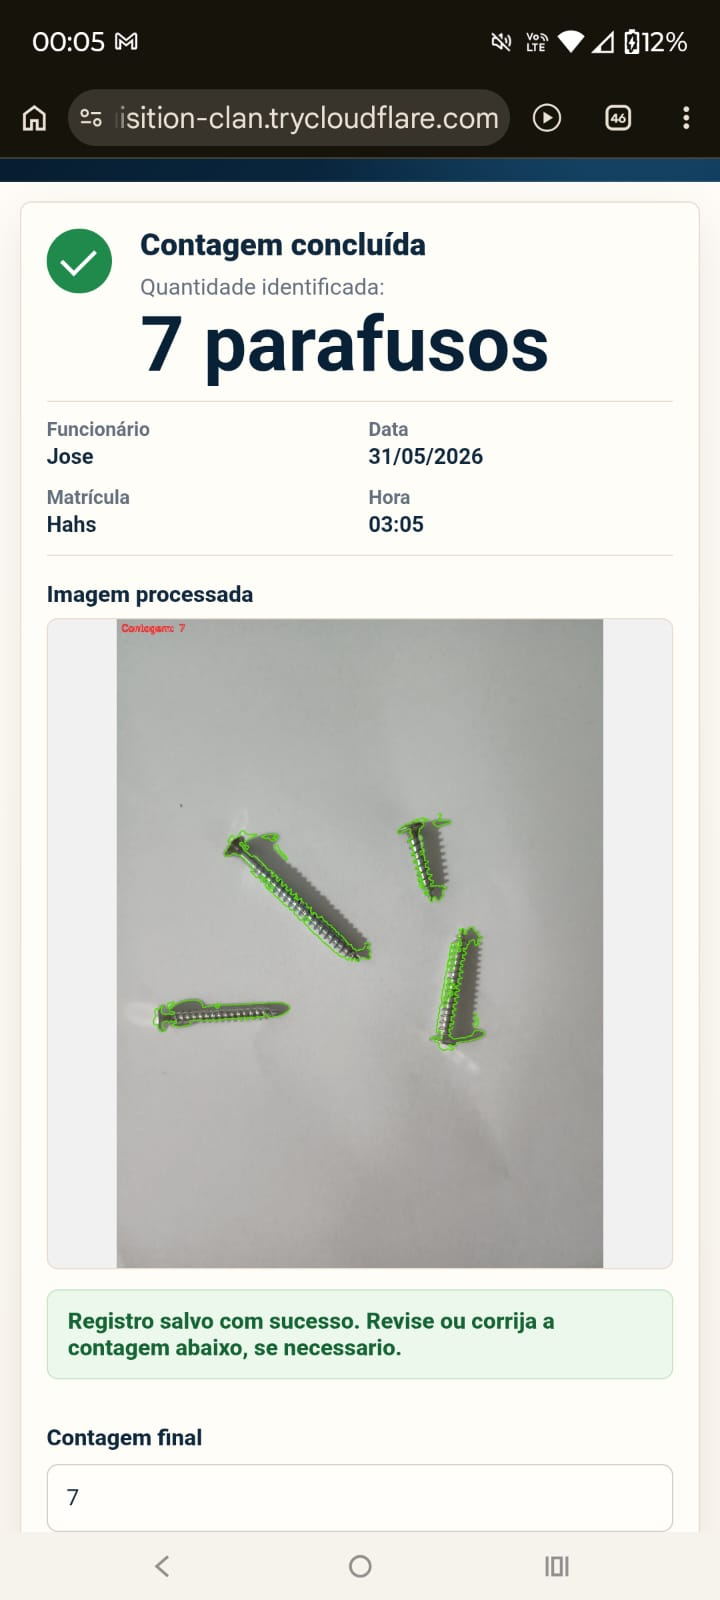
\includegraphics[width=\linewidth]{opencv1.jpeg}
    \caption{Resultado OpenCV -- imagem 1}
  \end{subfigure}\hfill
  \begin{subfigure}[t]{0.31\textwidth}
    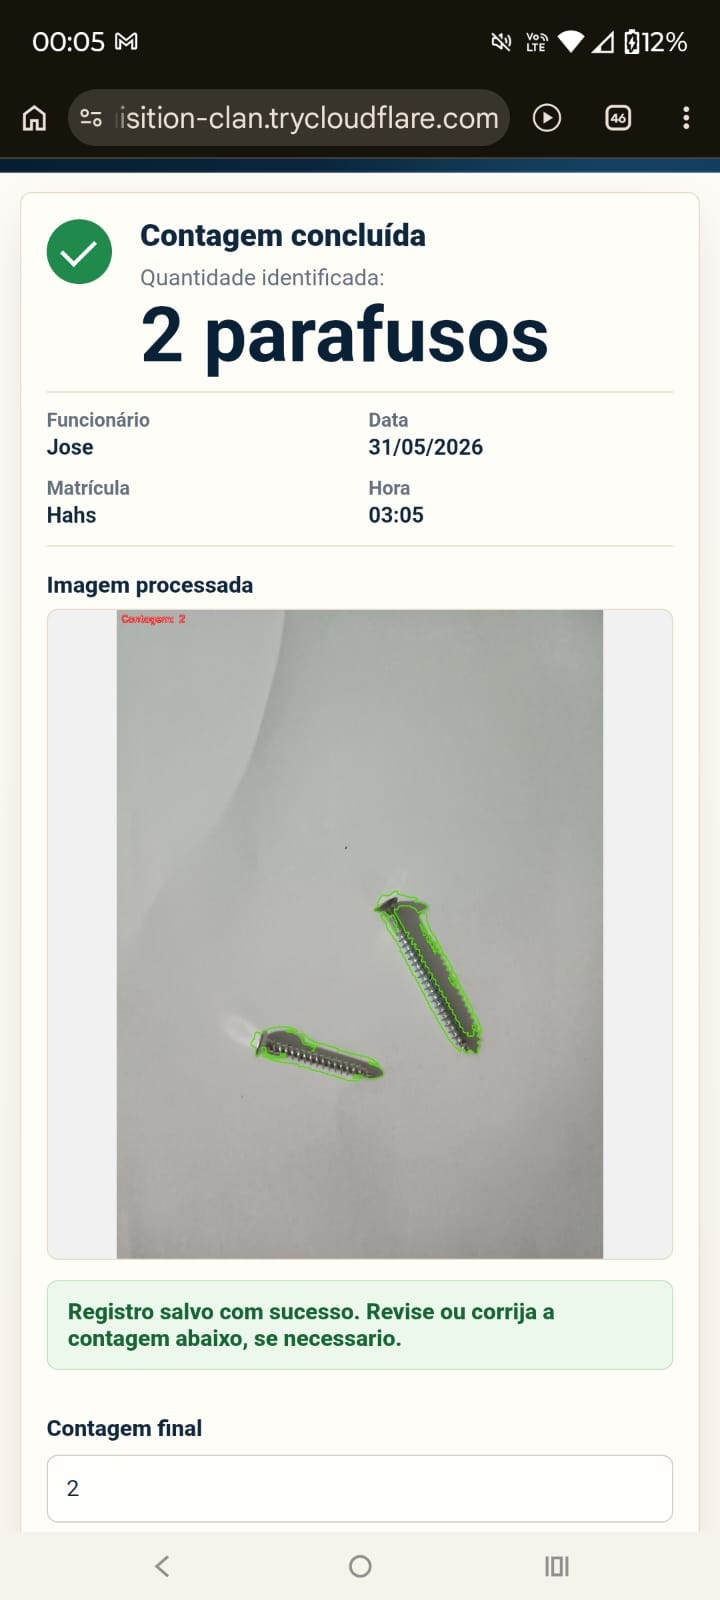
\includegraphics[width=\linewidth]{opencv2.jpeg}
    \caption{Resultado OpenCV -- imagem 2}
  \end{subfigure}\hfill
  \begin{subfigure}[t]{0.31\textwidth}
    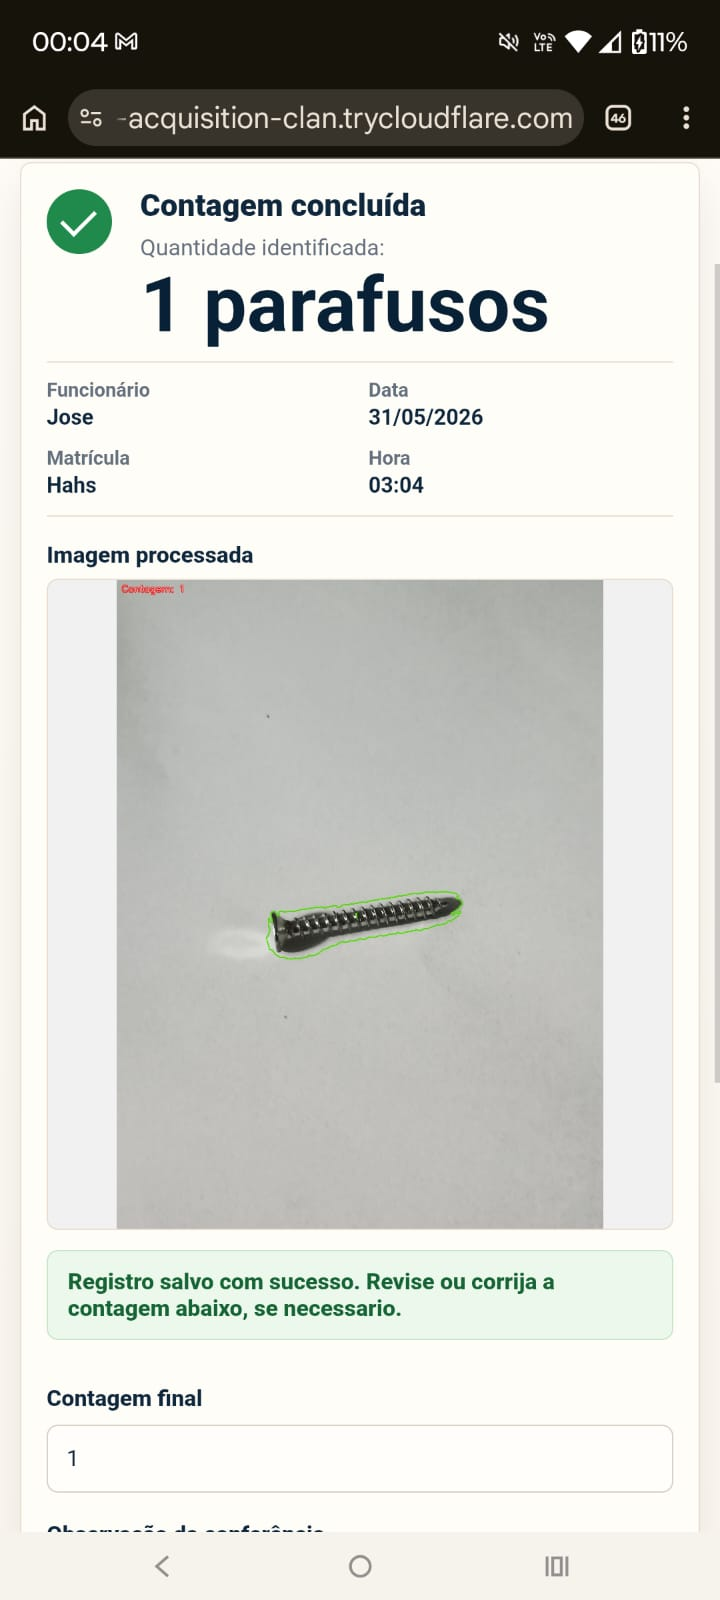
\includegraphics[width=\linewidth]{opencv3.jpeg}
    \caption{Resultado OpenCV -- imagem 3}
  \end{subfigure}
  \caption{Resultados pr\'aticos do pipeline cl\'assico em novas imagens.}
  \label{fig:opencv-resultados}
\end{figure}

\subsection{Grade de Debug -- Pipeline Interno}

A Figura~\ref{fig:grid-debug} exibe a grade de debug gerada pela fun\c{c}\~ao
\texttt{make\_debug\_grid}, mostrando os est\'agios internos do pipeline: imagem
original, pr\'e-processada (CLAHE), m\'ascara bin\'aria, \emph{distance transform},
mapa de picos (watershed) e imagem anotada final. Esta visualiza\c{c}\~ao \'e
fundamental para auditar e depurar casos-limite.

\begin{figure}[H]
  \centering
  \begin{subfigure}[t]{0.48\textwidth}
    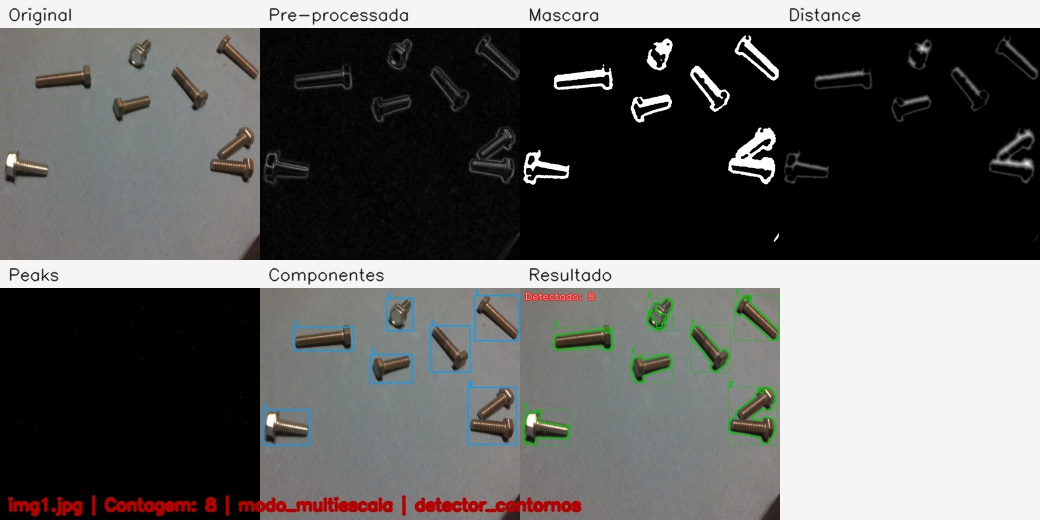
\includegraphics[width=\linewidth]{img1_debug.jpg}
    \caption{Debug -- imagem 1}
  \end{subfigure}\hfill
  \begin{subfigure}[t]{0.48\textwidth}
    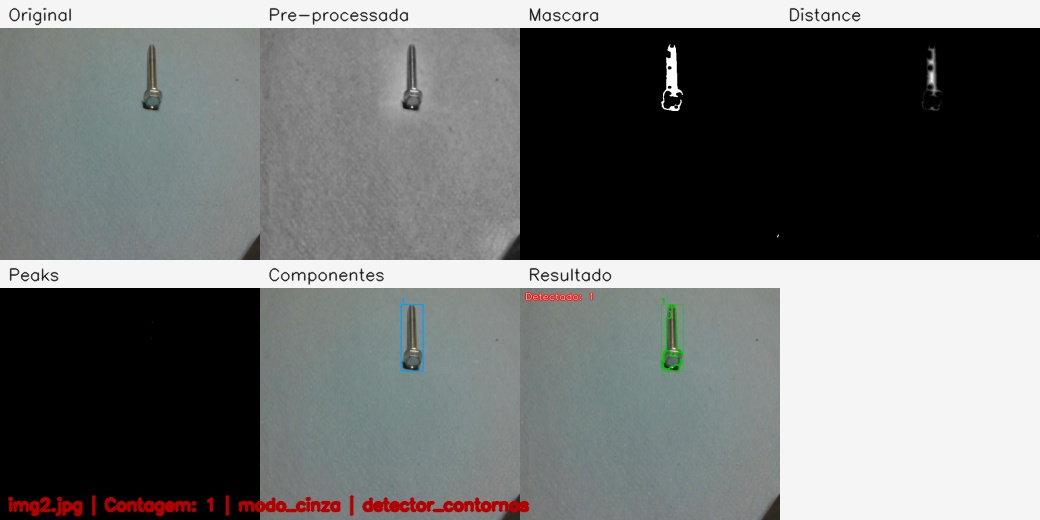
\includegraphics[width=\linewidth]{img2_debug.jpg}
    \caption{Debug -- imagem 2}
  \end{subfigure}

  \vspace{0.5em}
  \begin{subfigure}[t]{0.48\textwidth}
    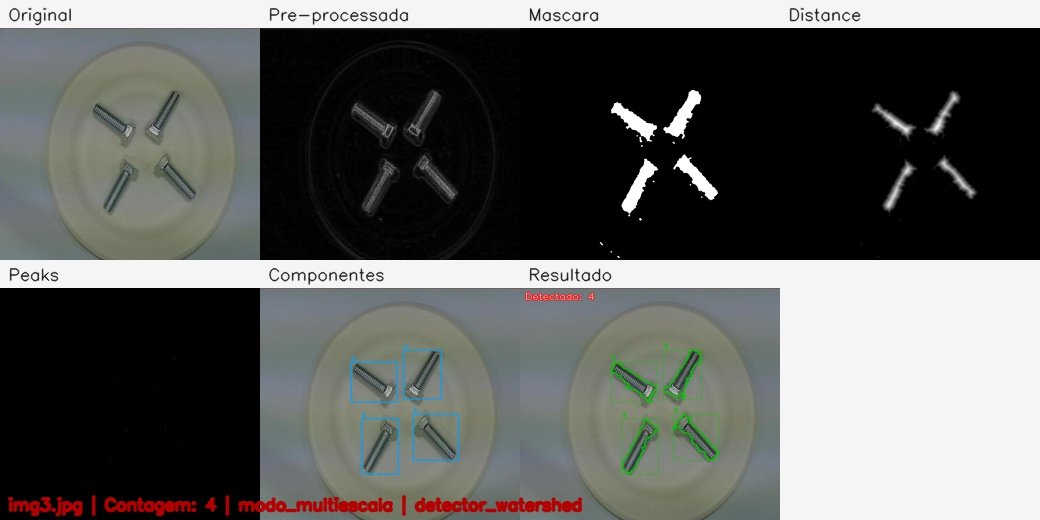
\includegraphics[width=\linewidth]{img3_debug.jpg}
    \caption{Debug -- imagem 3}
  \end{subfigure}\hfill
  \begin{subfigure}[t]{0.48\textwidth}
    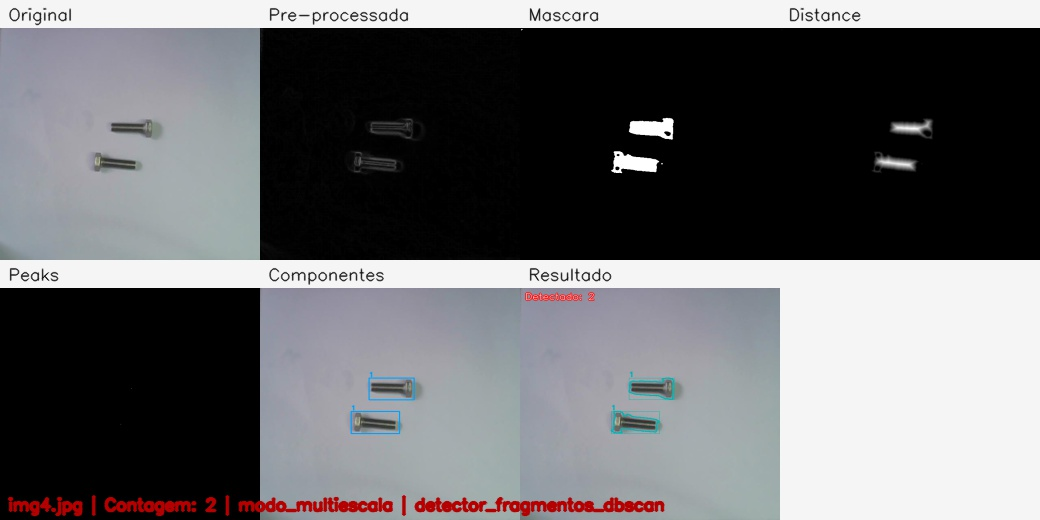
\includegraphics[width=\linewidth]{img4_debug.jpg}
    \caption{Debug -- imagem 4}
  \end{subfigure}

  \vspace{0.5em}
  \begin{subfigure}[t]{0.48\textwidth}
    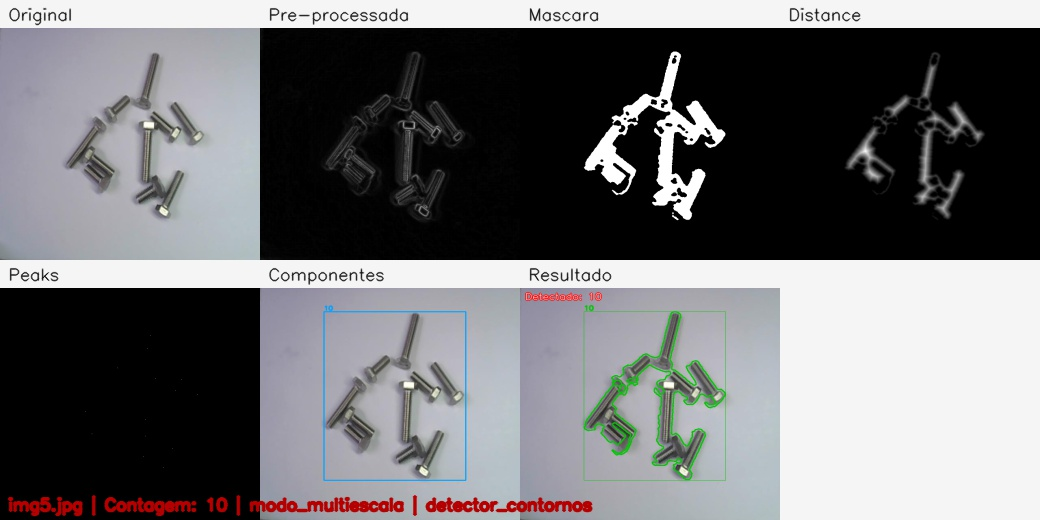
\includegraphics[width=\linewidth]{img5_debug.jpg}
    \caption{Debug -- imagem 5}
  \end{subfigure}\hfill
  \begin{subfigure}[t]{0.48\textwidth}
    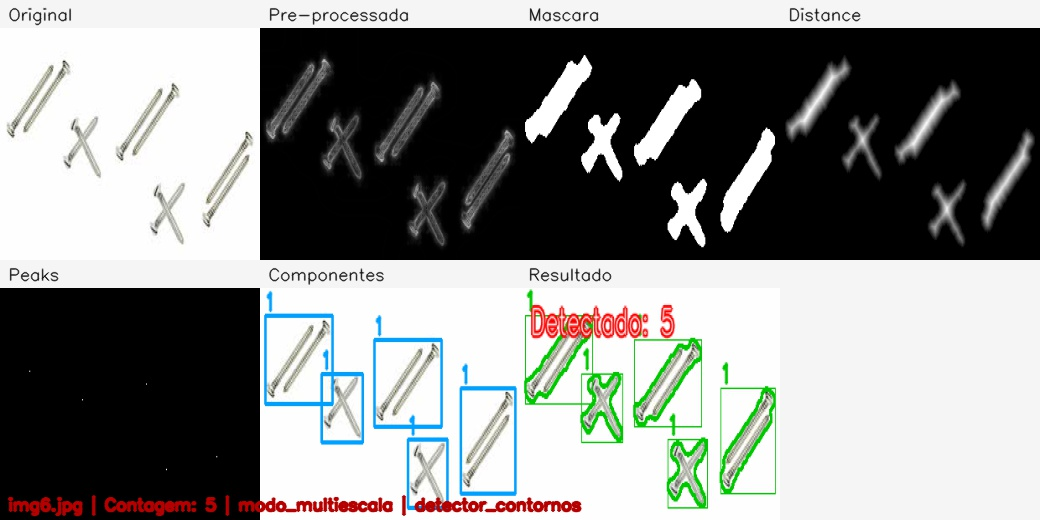
\includegraphics[width=\linewidth]{img6_debug.jpg}
    \caption{Debug -- imagem 6}
  \end{subfigure}
  \caption{Grades de debug do pipeline cl\'assico: cada painel exibe os est\'agios de
           pr\'e-processamento, segmenta\c{c}\~ao, \emph{distance transform} e resultado.}
  \label{fig:grid-debug}
\end{figure}

\subsection{M\'etricas de Avalia\c{c}\~ao -- Vis\~ao Cl\'assica}

As Figuras~\ref{fig:avaliacao-v3} e~\ref{fig:discriminacao-v3} apresentam, respectivamente,
o painel de avalia\c{c}\~ao quantitativa (MAE, acur\'acia exata e vi\'es por imagem) e a
an\'alise de discrimina\c{c}\~ao de \emph{features} usadas pelo classificador de cena.

\begin{figure}[H]
  \centering
  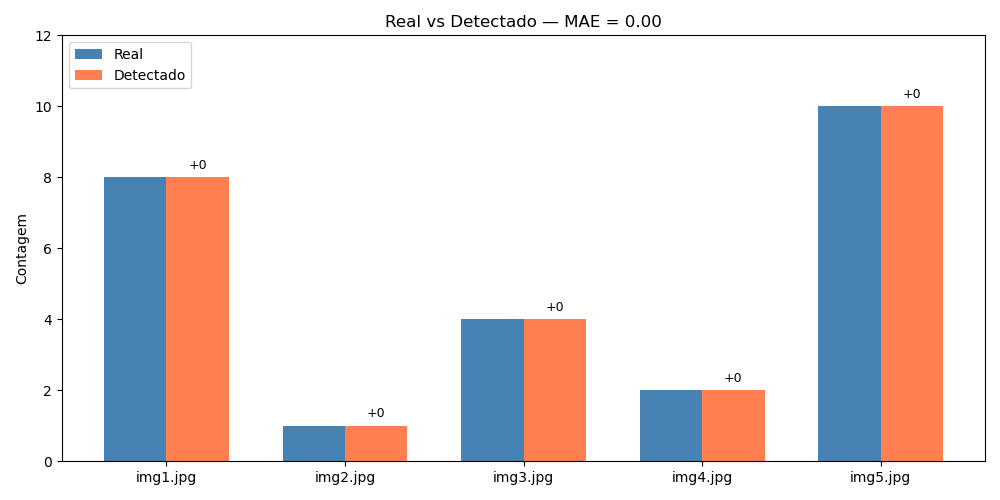
\includegraphics[width=0.96\linewidth]{avaliacao_v3.png}
  \caption{Painel de avalia\c{c}\~ao quantitativa da Solu\c{c}\~ao 1: MAE, acur\'acia
           exata e erros assinados por imagem.}
  \label{fig:avaliacao-v3}
\end{figure}

\begin{figure}[H]
  \centering
  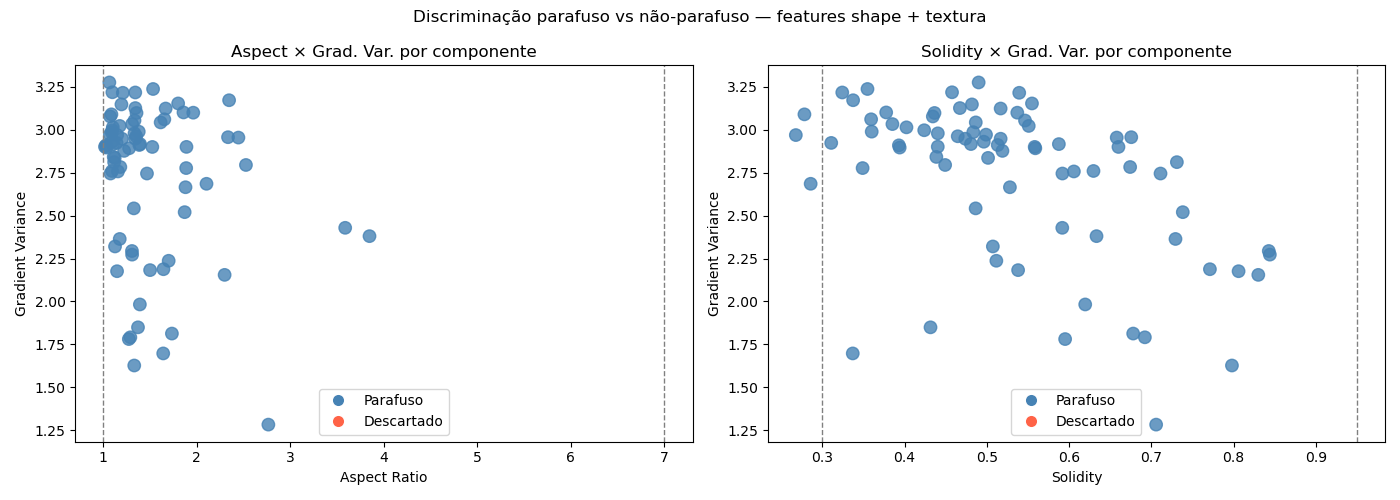
\includegraphics[width=0.96\linewidth]{discriminacao_features_v3.png}
  \caption{An\'alise das \emph{features} de discrimina\c{c}\~ao de cena usadas pelo
           \texttt{classify\_scene}: brilho, contraste, textura e densidade.}
  \label{fig:discriminacao-v3}
\end{figure}

\subsection{Grid de Resultados Consolidado}

A Figura~\ref{fig:grid-v3} apresenta o painel consolidado com todos os resultados
de contagem do pipeline cl\'assico sobre o conjunto de imagens avaliado, permitindo
visualizar de forma comparativa o desempenho em diferentes cen\'arios.

\begin{figure}[H]
  \centering
  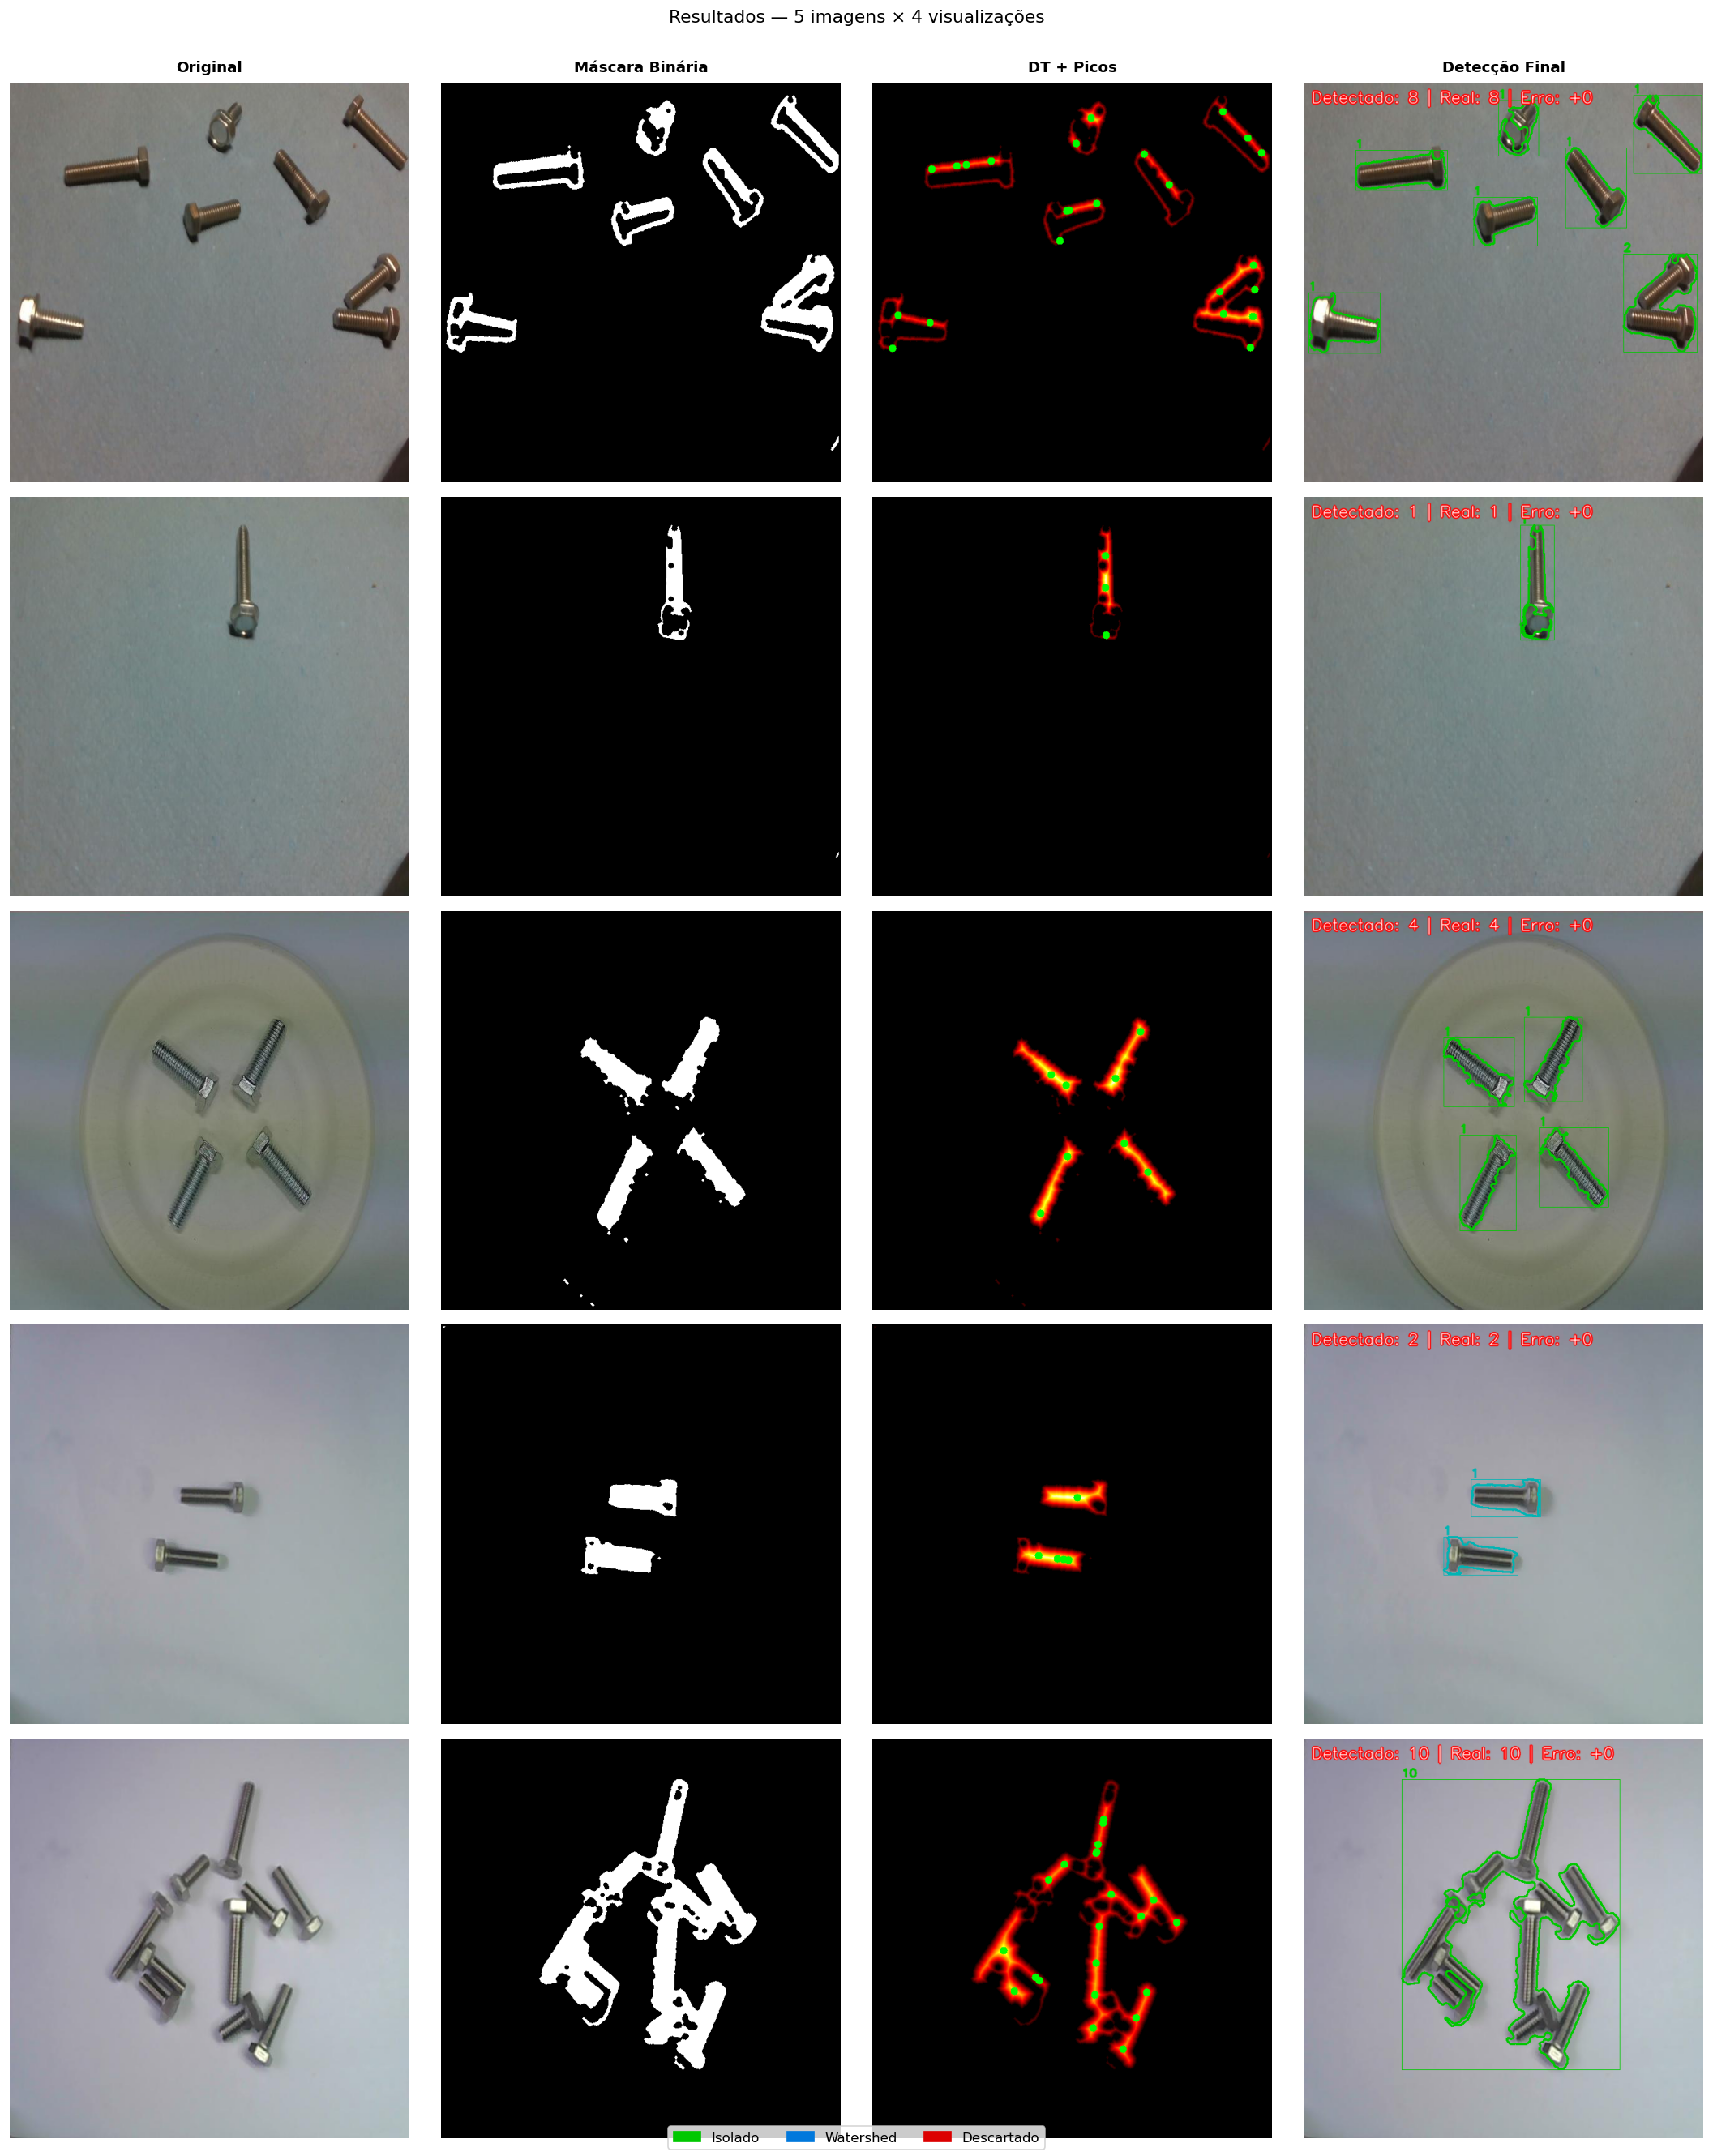
\includegraphics[width=\linewidth]{grid_resultados_v3.png}
  \caption{Grid consolidado de resultados da Solu\c{c}\~ao 1 (Vis\~ao Cl\'assica):
           contagem detectada \textit{vs.} contagem real em cada imagem avaliada.}
  \label{fig:grid-v3}
\end{figure}

%% ============================================================
\section{Solu\c{c}\~ao 2 -- Detec\c{c}\~ao com YOLOv11}
\label{sec:sol2}

\subsection{Motiva\c{c}\~ao}

Enquanto a Solu\c{c}\~ao 1 usa regras expl\'icitas, a Solu\c{c}\~ao 2 aprende
diretamente dos dados. O YOLOv11 foi escolhido por:

\begin{itemize}[leftmargin=*]
  \item Excelente equil\'ibrio entre velocidade de infer\^encia e precis\~ao.
  \item Suporte oficial a exporta\c{c}\~ao m\'ovel (\texttt{TFLite}, \texttt{NCNN},
        \texttt{CoreML}).
  \item Transfer learning a partir de pesos COCO reduz dados necess\'arios.
  \item API Python limpa do Ultralytics, f\'acil de integrar.
\end{itemize}

\subsection{Dataset}

O dataset utilizado foi o \textbf{Screw v4} do Roboflow, com anotac\~oes poligonais
convertidas para \emph{bounding boxes} pelo script
\texttt{scripts/convert\_segments\_to\_boxes.py}. H\'a uma \'unica classe:
\texttt{parafuso}.

\begin{lstlisting}[caption={Configura\c{c}\~ao do dataset (\texttt{data.yaml})}]
path: ../Screw.v4-dataset-screw4.yolov11
train: train/images
val:   valid/images
test:  test/images
names:
  0: parafuso
\end{lstlisting}

\subsection{Treinamento}

O script \texttt{scripts/train\_screws\_yolo.py} encapsula o ciclo completo de
treinamento com detec\c{c}\~ao autom\'atica de GPU e gera\c{c}\~ao de
\texttt{data.ultralytics.yaml} com caminhos absolutos (solu\c{c}\~ao para
problema de path no Windows).

\begin{lstlisting}[caption={Treinamento do modelo YOLOv11}]
model = YOLO("yolo11s.pt")   # Transfer learning de COCO
model.train(
    data=str(train_yaml),
    epochs=100,
    imgsz=768,       # Equilibrio velocidade/precisao
    batch=4,         # Limitacao de memoria GPU
    patience=30,     # Early stopping
    device=0,        # GPU CUDA
    close_mosaic=10, # Estabiliza convergencia final
    amp=True,        # Precisao mista (mais rapido)
)
\end{lstlisting}

A Tabela~\ref{tab:runs} resume as configura\c{c}\~oes avaliadas:

\begin{table}[H]
  \centering
  \caption{Execu\c{c}\~oes de treinamento avaliadas}
  \label{tab:runs}
  \begin{tabular}{lcccc}
    \toprule
    \textbf{Execu\c{c}\~ao} & \textbf{Modelo} & \textbf{imgsz} &
    \textbf{\'Epocas} & \textbf{Selecionado} \\
    \midrule
    \texttt{yolo11\_screws}       & yolo11s.pt & 960  & 100 & \\
    \texttt{yolo11\_screws-2}     & yolo11s.pt & 768  & 100 & \checkmark \\
    \texttt{yolo11\_screws\_combined} & yolo11s.pt & 1280 & 100 & \\
    \texttt{yolo11\_screws\_hard} & yolo11s.pt & 960  & 100 & \\
    \bottomrule
  \end{tabular}
\end{table}

\subsection{M\'odulo de Infer\^encia}

A fun\c{c}\~ao \texttt{contar\_parafusos} em \texttt{screw\_counter.py} implementa
um \emph{cache} global de modelo para evitar recarregamento em cada requisi\c{c}\~ao:

\begin{lstlisting}[caption={Infer\^encia com cache de modelo (\texttt{screw\_counter.py})}]
_MODEL_CACHE: dict[str, YOLO] = {}   # Carrega uma vez, reutiliza sempre

def contar_parafusos(image_path, model_path, output_dir,
                     conf=0.25, iou=0.45, imgsz=None, ...):
    # Cache: evita overhead de 1-3s por requisicao
    model_key = str(model_path.resolve())
    if model_key not in _MODEL_CACHE:
        _MODEL_CACHE[model_key] = YOLO(model_key)
    model = _MODEL_CACHE[model_key]

    results = model.predict(source=str(image_path),
                            conf=conf, iou=iou, verbose=False)
    boxes = results[0].boxes
    total = 0 if boxes is None else len(boxes)
    # Anota imagem e retorna payload completo
    ...
\end{lstlisting}

\subsection{Hiperpar\^ametros de Infer\^encia}

\begin{table}[H]
  \centering
  \caption{Par\^ametros de infer\^encia e sua justificativa}
  \label{tab:hiper}
  \begin{tabular}{lll}
    \toprule
    \textbf{Par\^ametro} & \textbf{Valor} & \textbf{Justificativa} \\
    \midrule
    \texttt{CONF\_THRESHOLD} & 0.25 & Equil\'ibrio precision/recall \\
    \texttt{IOU\_THRESHOLD}  & 0.45 & Evita detec\c{c}\~oes duplicadas \\
    \texttt{DEFAULT\_IMGSZ}  & 1280 & Alta resolu\c{c}\~ao p/ parafusos pequenos \\
    \bottomrule
  \end{tabular}
\end{table}

\subsection{Exporta\c{c}\~ao Mobile}

Scripts dedicados convertem o modelo para formatos otimizados:

\begin{itemize}[leftmargin=*]
  \item \texttt{export\_tflite.py} -- Android (quantiza\c{c}\~ao INT8)
  \item \texttt{export\_ncnn.py}  -- Android/ARM (engine ultra-leve)
  \item \texttt{export\_coreml.py} -- iOS (Neural Engine da Apple)
\end{itemize}

\begin{tcolorbox}[vantagem={Vantagens da Solu\c{c}\~ao 2}]
\begin{itemize}[leftmargin=*, noitemsep]
  \item Robusta a varia\c{c}\~oes de ilumina\c{c}\~ao, fundo e orienta\c{c}\~ao.
  \item Lida bem com parafusos sobrepostos (NMS por IoU).
  \item Localiza\c{c}\~ao precisa de cada inst\^ancia (bounding box).
  \item Generaliza para novos cen\'arios ap\'os fino ajuste (\emph{fine-tuning}).
  \item Exporta\c{c}\~ao nativa para smartphones via TFLite/NCNN.
\end{itemize}
\end{tcolorbox}

%% --- Metricas de validacao YOLO (numeros reais verificados) ---
\subsection{M\'etricas de Valida\c{c}\~ao -- Resultados Quantitativos}
\label{sec:metricas-yolo}

\subsubsection{M\'etodo de Valida\c{c}\~ao Empregado}

A valida\c{c}\~ao foi conduzida com o m\'etodo \texttt{model.val()} do Ultralytics,
encapsulado no script \texttt{scripts/validate\_screws\_yolo.py}. O modelo \'e avaliado
sobre o conjunto de valida\c{c}\~ao (\texttt{valid/images}), \textbf{separado} do conjunto
de treino, garantindo que as m\'etricas reflitam a capacidade de \textbf{generaliza\c{c}\~ao}
do modelo. As m\'etricas seguem o protocolo padr\~ao de detec\c{c}\~ao de objetos (COCO):

\begin{lstlisting}[caption={Extra\c{c}\~ao das m\'etricas de valida\c{c}\~ao (\texttt{validate\_screws\_yolo.py})}]
model = YOLO(str(model_path))
metrics = model.val(data=str(val_yaml), conf=args.conf)

precision = float(metrics.box.mp)    # Precision media
recall    = float(metrics.box.mr)    # Recall medio
map50     = float(metrics.box.map50) # mAP @ IoU=0.50
map5095   = float(metrics.box.map)   # mAP @ IoU=0.50:0.95
\end{lstlisting}

\begin{description}[leftmargin=*, style=nextline]
  \item[Precision (P):] propor\c{c}\~ao de detec\c{c}\~oes corretas dentre todas as
    detec\c{c}\~oes feitas -- mede \emph{falsos positivos}.
  \item[Recall (R):] propor\c{c}\~ao de parafusos reais que foram detectados --
    mede \emph{falsos negativos}.
  \item[mAP50:] \emph{mean Average Precision} com IoU $\geq 0.50$; m\'etrica principal
    de refer\^encia.
  \item[mAP50-95:] m\'edia do mAP para IoU de $0.50$ a $0.95$ (passo $0.05$);
    m\'etrica mais rigorosa, que penaliza localiza\c{c}\~ao imprecisa.
\end{description}

\subsubsection{Resultados Obtidos (Verificados)}

A Tabela~\ref{tab:metricas-reais} apresenta as m\'etricas reais de valida\c{c}\~ao,
extra\'idas diretamente do relat\'orio gerado pelo script de valida\c{c}\~ao
(\texttt{validation\_report.txt}) sobre os pesos \texttt{best.pt} do modelo de produ\c{c}\~ao
(\texttt{yolo11\_screws-2}).

\begin{table}[H]
  \centering
  \caption{M\'etricas de valida\c{c}\~ao do modelo YOLOv11 \texttt{yolo11\_screws-2}
           (sa\'ida oficial de \texttt{model.val()})}
  \label{tab:metricas-reais}
  \renewcommand{\arraystretch}{1.3}
  \begin{tabular}{lcl}
    \toprule
    \textbf{M\'etrica} & \textbf{Valor} & \textbf{Interpreta\c{c}\~ao} \\
    \midrule
    Precision (P) & \textbf{0,9821} & 98,2\% das detec\c{c}\~oes est\~ao corretas \\
    Recall (R)    & \textbf{0,9776} & 97,8\% dos parafusos reais s\~ao detectados \\
    mAP50         & \textbf{0,9878} & desempenho geral (IoU $\geq$ 0,50) \\
    mAP50-95      & \textbf{0,9485} & localiza\c{c}\~ao das caixas \\
    \bottomrule
  \end{tabular}
\end{table}

\begin{tcolorbox}[vantagem={Leitura dos Resultados}]
Os valores indicam um modelo \textbf{maduro e preciso}: com
\textbf{mAP50 de 98,8\%} e precision/recall ambos acima de 97\%, o sistema erra muito
pouco -- tanto por excesso (falsos parafusos) quanto por falta (parafusos perdidos) --
exatamente o equil\'ibrio necess\'ario para uma contagem confi\'avel no processo de
\emph{picking}. O \textbf{mAP50-95 de 94,9\%} confirma que as caixas n\~ao apenas
detectam, mas \textbf{localizam com alta precis\~ao} cada parafuso, mesmo sob crit\'erios
rigorosos de sobreposi\c{c}\~ao.
\end{tcolorbox}

\medskip
\textit{Observa\c{c}\~ao sobre reprodutibilidade:} as m\'etricas reportadas correspondem
\`a sa\'ida oficial do procedimento \texttt{model.val()} registrada em
\texttt{validation\_report.txt}, sobre o conjunto de valida\c{c}\~ao separado do treino.
Pequenas varia\c{c}\~oes podem ocorrer entre execu\c{c}\~oes devido a diferen\c{c}as de
\texttt{conf}, \texttt{imgsz} e vers\~ao do Ultralytics; por isso, adotou-se sempre a
sa\'ida do script de valida\c{c}\~ao como fonte \'unica de verdade.

%% --- Curvas de treinamento YOLO ---
\subsection{Curvas de Treinamento -- Evolu\c{c}\~ao por \'Epoca}

A seguir s\~ao apresentadas as curvas de treinamento geradas automaticamente pelo
Ultralytics ao longo das 100 \'epocas de treinamento do modelo.

\begin{figure}[H]
  \centering
  \begin{subfigure}[t]{0.48\textwidth}
    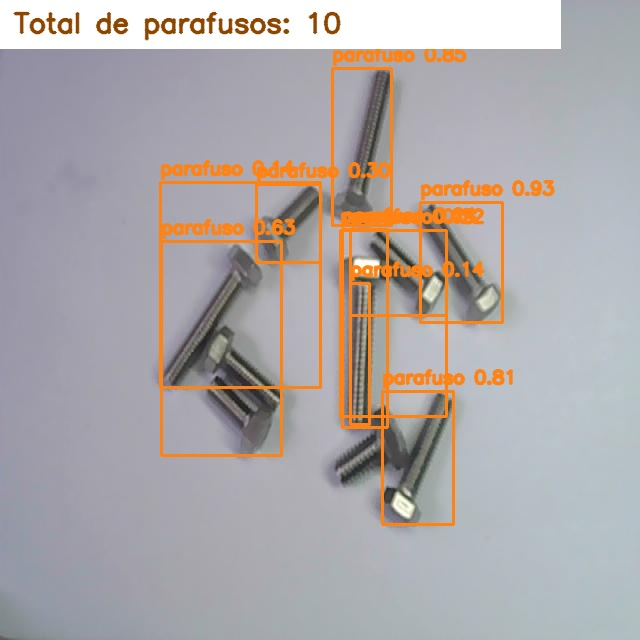
\includegraphics[width=\linewidth]{treinamento-yolo1.jpg}
    \caption{Curvas de perda de \emph{box}, classifica\c{c}\~ao e DFL}
  \end{subfigure}\hfill
  \begin{subfigure}[t]{0.48\textwidth}
    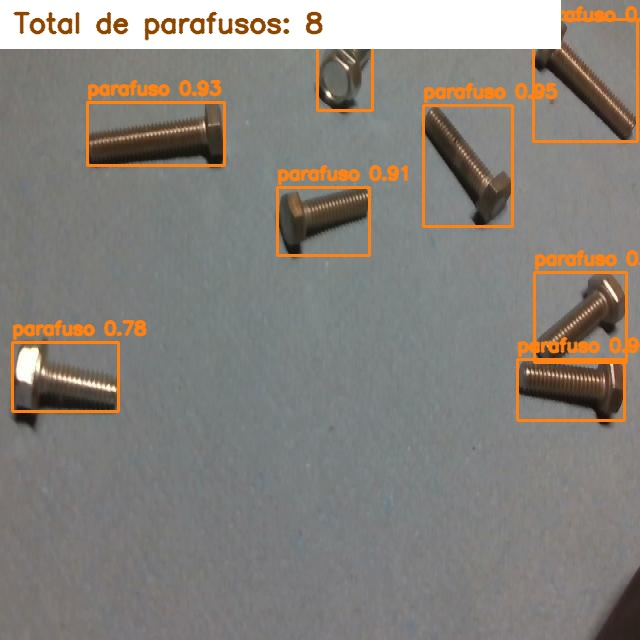
\includegraphics[width=\linewidth]{treinamento-yolo2.jpg}
    \caption{M\'etricas de valida\c{c}\~ao: precision, recall, mAP50 e mAP50-95}
  \end{subfigure}

  \vspace{0.5em}
  \begin{subfigure}[t]{0.48\textwidth}
    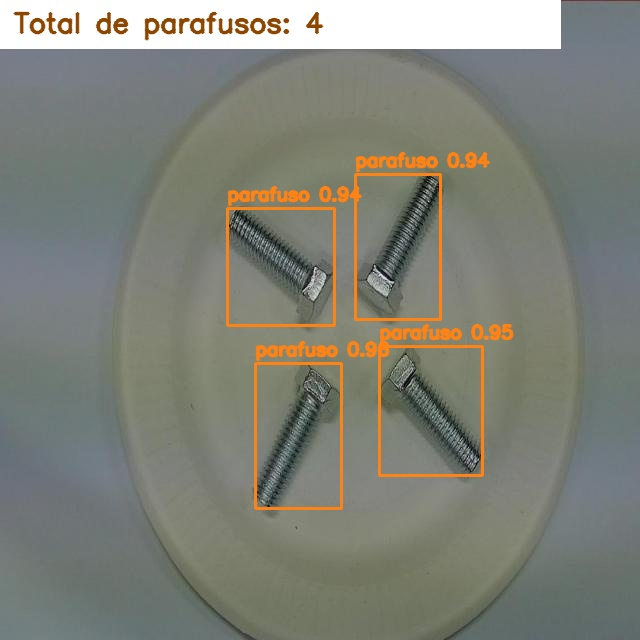
\includegraphics[width=\linewidth]{treinamento-yolo3.jpg}
    \caption{Evolu\c{c}\~ao do mAP ao longo das \'epocas}
  \end{subfigure}\hfill
  \begin{subfigure}[t]{0.48\textwidth}
    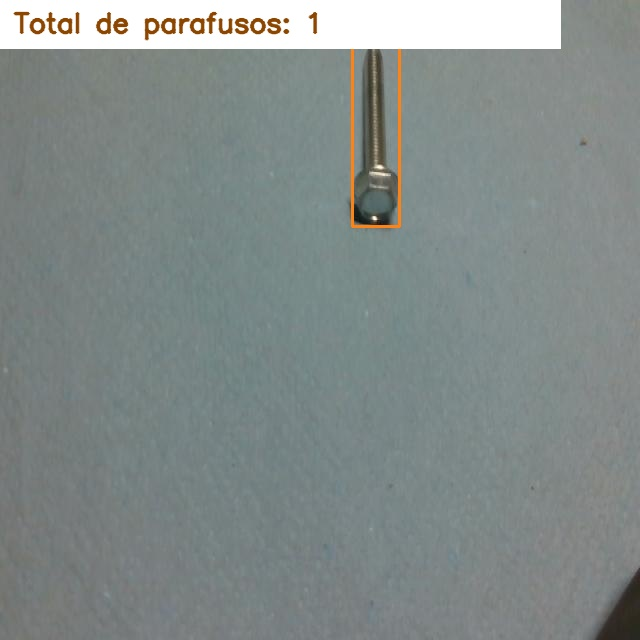
\includegraphics[width=\linewidth]{treinamento-yoo4.jpg}
    \caption{Taxa de aprendizado e \emph{warmup}}
  \end{subfigure}
  \caption{Curvas de treinamento do YOLOv11 (\texttt{yolo11\_screws-2}, 100 \'epocas,
           \texttt{imgsz=768}, GPU CUDA).}
  \label{fig:yolo-treino}
\end{figure}

\subsection{Matriz de Confus\~ao}

A matriz de confus\~ao \'e a principal ferramenta para avaliar se o modelo comete erros
de \emph{falso positivo} (detecta parafuso onde n\~ao h\'a) ou \emph{falso negativo}
(n\~ao detecta um parafuso presente). A Figura~\ref{fig:conf-matrix} apresenta as
vers\~oes absoluta e normalizada.

\begin{figure}[H]
  \centering
  \begin{subfigure}[t]{0.48\textwidth}
    
\includegraphics[width=\linewidth]{confusion_matrix.png}
    \caption{Matriz de confus\~ao (valores absolutos)}
  \end{subfigure}\hfill
  \begin{subfigure}[t]{0.48\textwidth}
    
\includegraphics[width=\linewidth]{confusion_matrix_normalized.png}
    \caption{Matriz de confus\~ao normalizada}
  \end{subfigure}
  \caption{Matrizes de confus\~ao do YOLOv11 sobre o conjunto de teste.
           A diagonal principal concentra as detec\c{c}\~oes corretas;
           elementos fora da diagonal representam erros de classifica\c{c}\~ao.}
  \label{fig:conf-matrix}
\end{figure}

\subsection{Curvas de Precis\~ao, Recall e F1}

As curvas de precis\~ao (P), recall (R), F1 e PR (\emph{Precision-Recall}) oferecem
uma vis\~ao completa do comportamento do modelo para diferentes limiares de confian\c{c}a.

\begin{figure}[H]
  \centering
  \begin{subfigure}[t]{0.48\textwidth}
    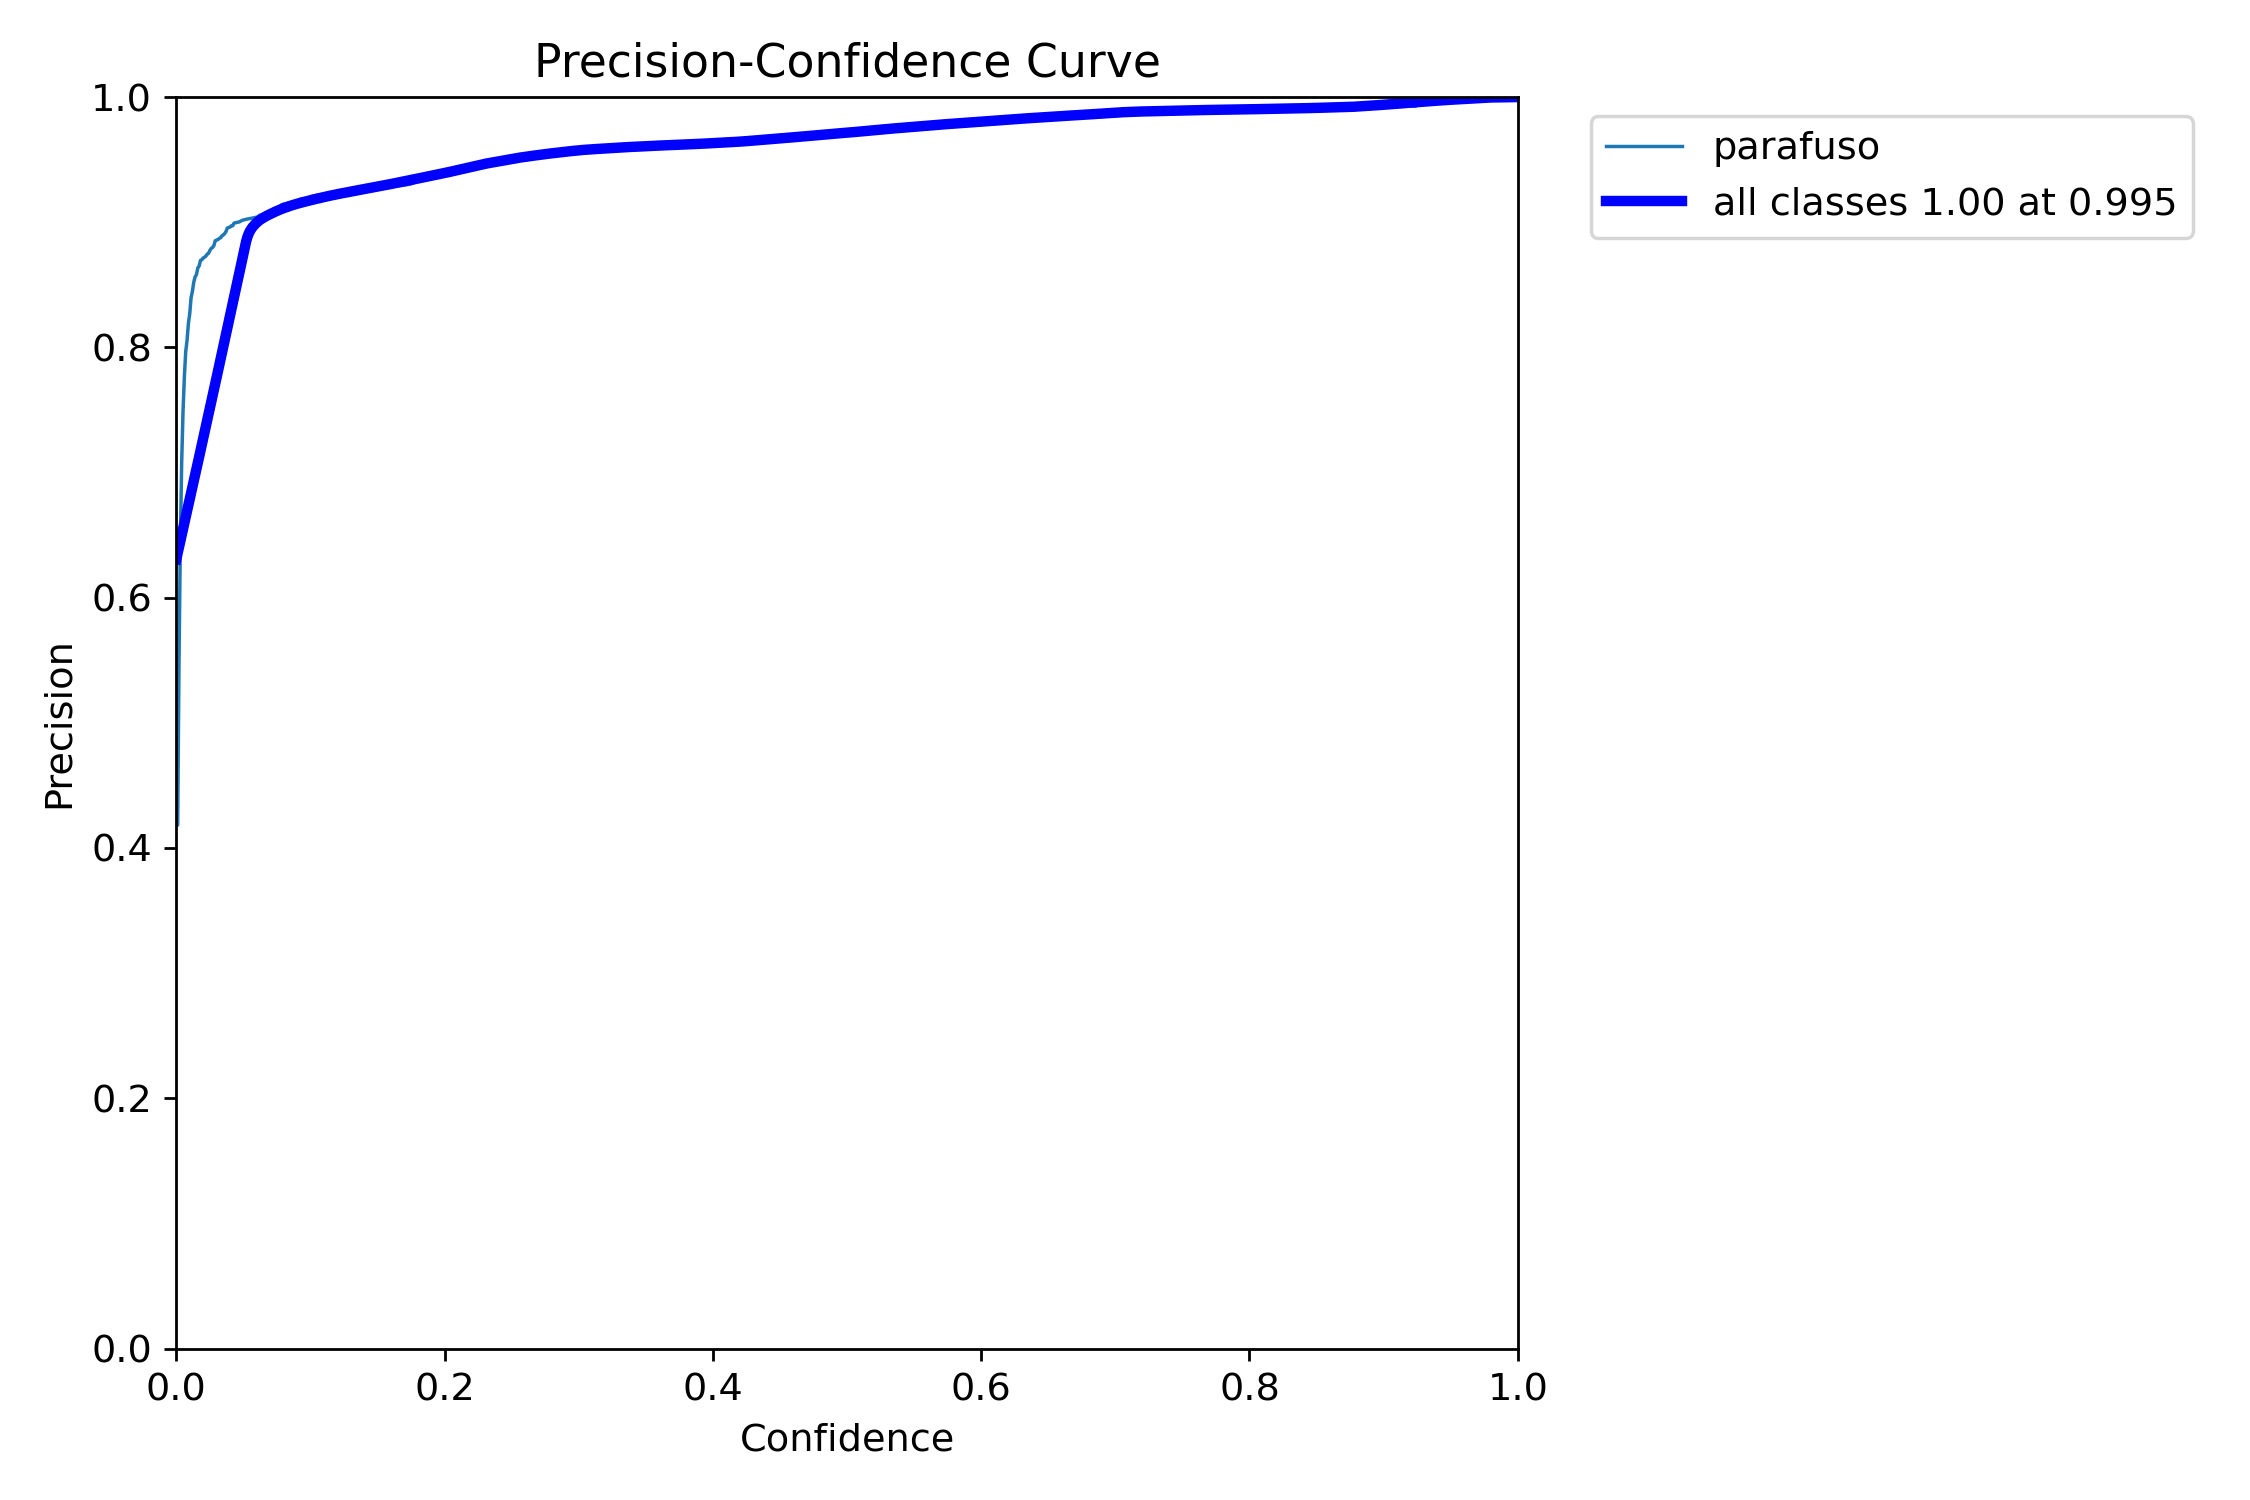
\includegraphics[width=\linewidth]{BoxP_curve.png}
    \caption{Curva de Precis\~ao (P)}
  \end{subfigure}\hfill
  \begin{subfigure}[t]{0.48\textwidth}
    
\includegraphics[width=\linewidth]{BoxR_curve.png}
    \caption{Curva de Recall (R)}
  \end{subfigure}

  \vspace{0.5em}
  \begin{subfigure}[t]{0.48\textwidth}
    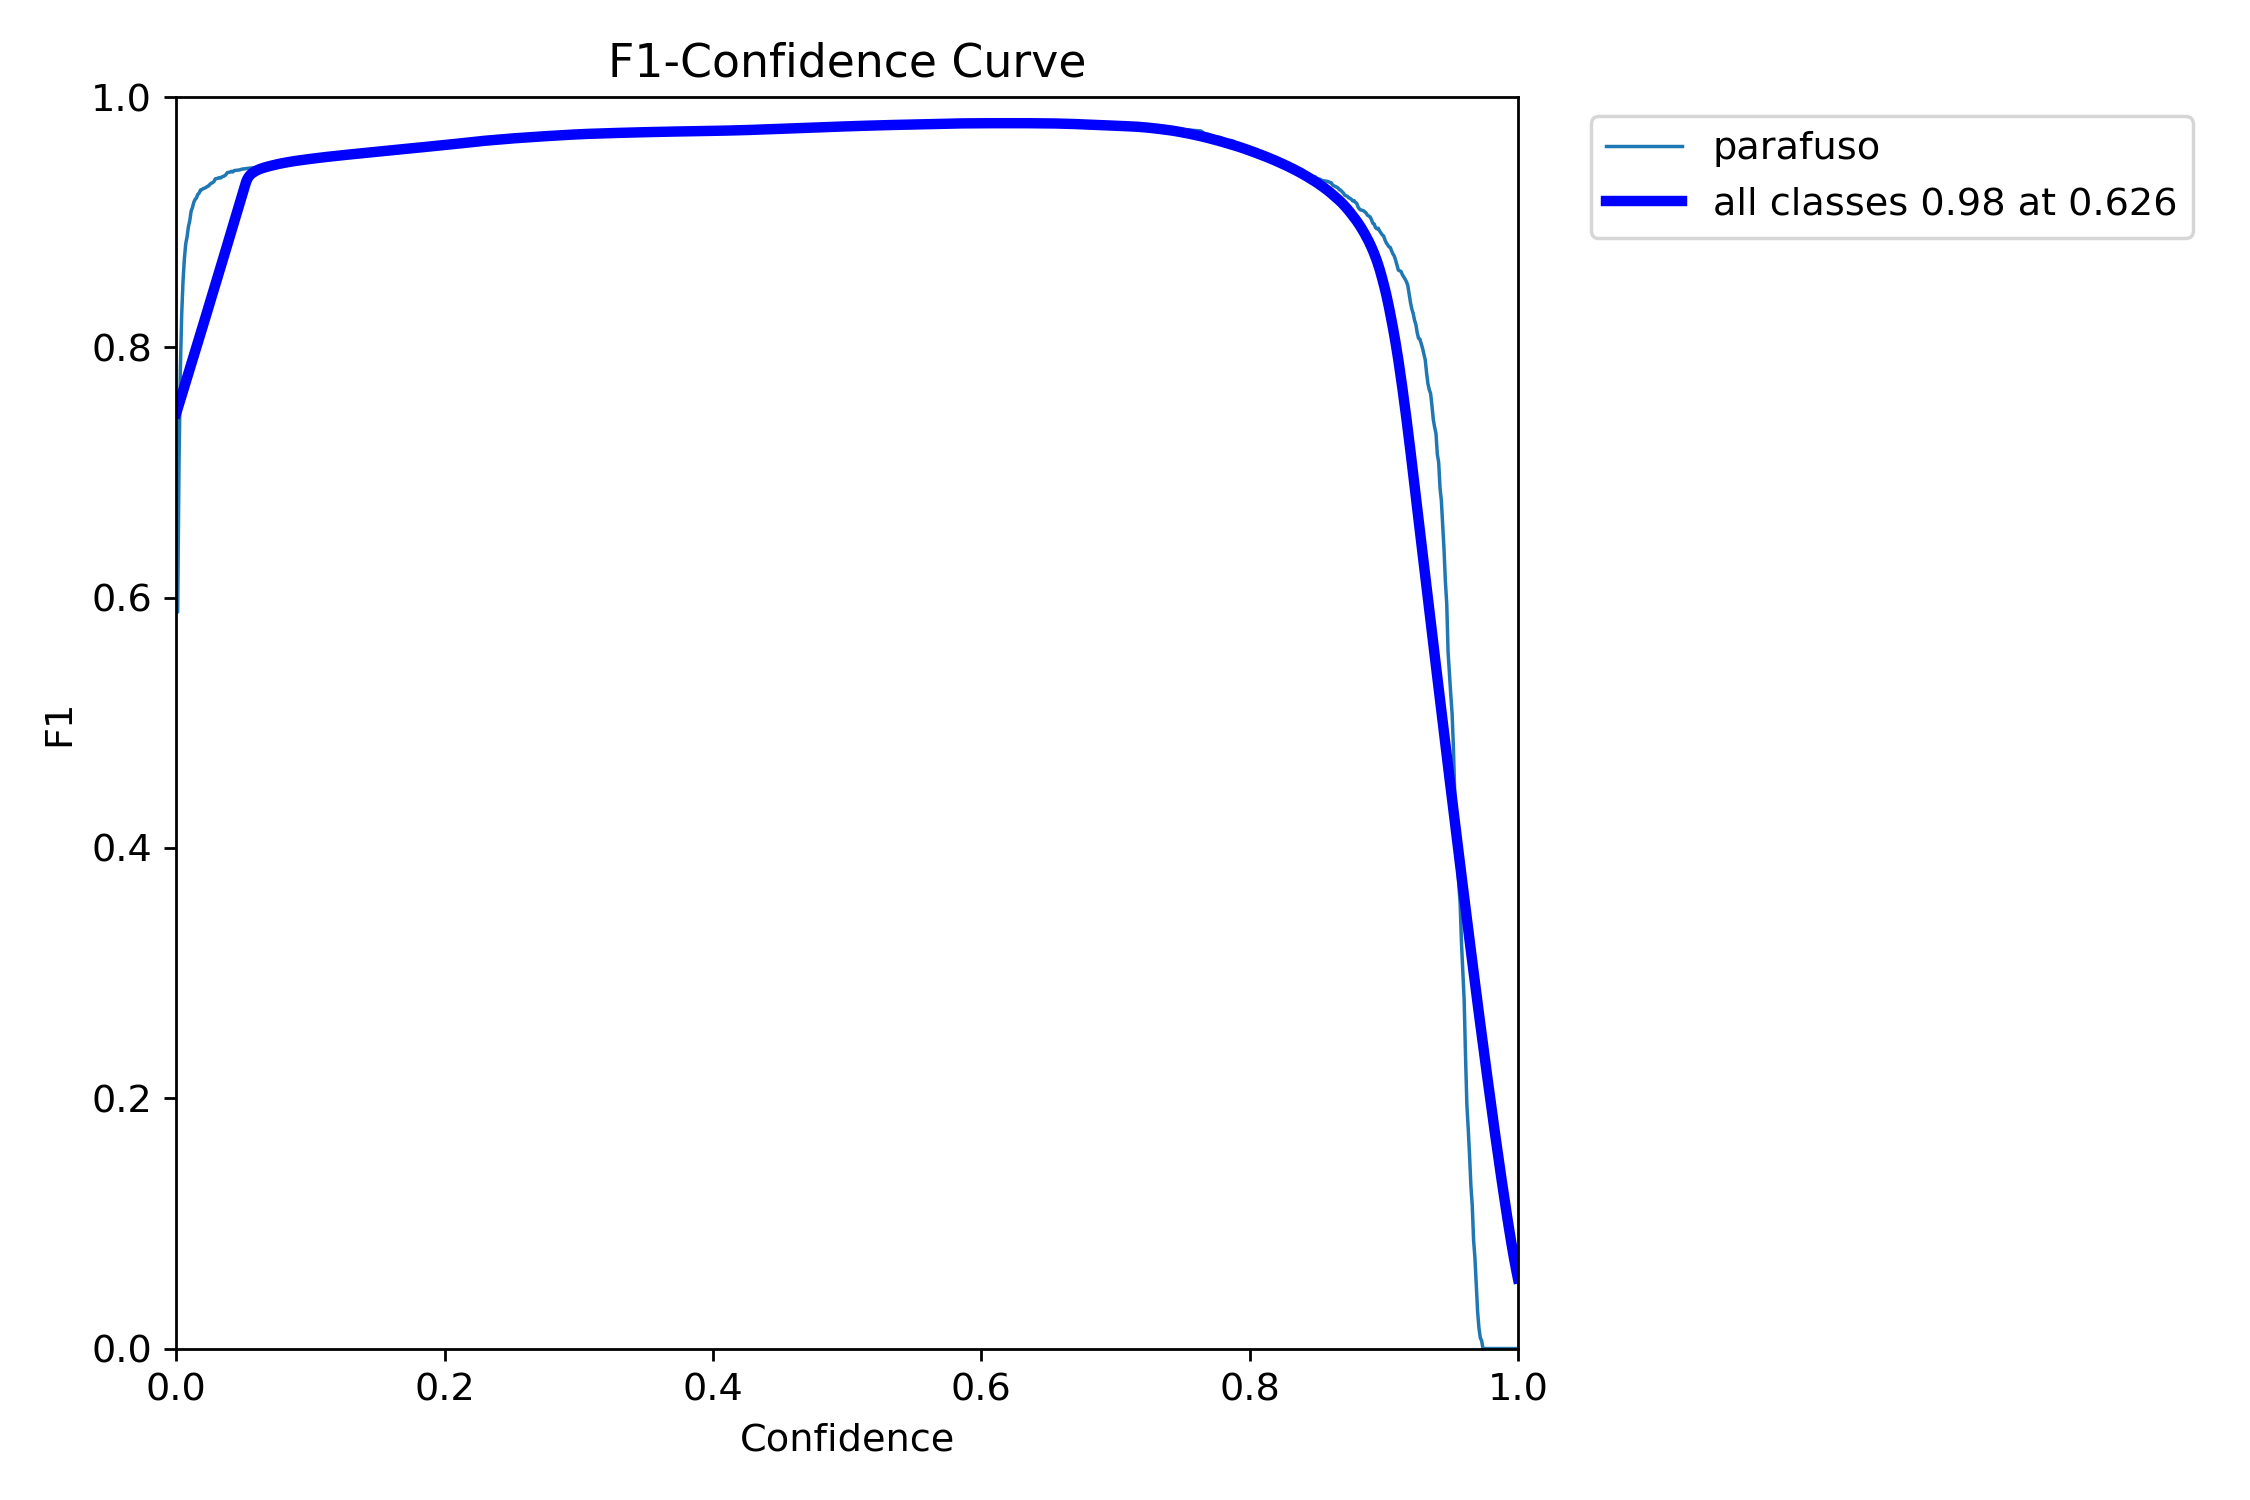
\includegraphics[width=\linewidth]{BoxF1_curve.png}
    \caption{Curva F1 \emph{vs.} limiar de confian\c{c}a}
  \end{subfigure}\hfill
  \begin{subfigure}[t]{0.48\textwidth}
    
\includegraphics[width=\linewidth]{BoxPR_curve.png}
    \caption{Curva PR (\emph{Precision-Recall})}
  \end{subfigure}
  \caption{Curvas de avalia\c{c}\~ao do YOLOv11 sobre o conjunto de valida\c{c}\~ao.
           O limiar \texttt{conf=0.25} foi selecionado a partir da an\'alise da
           curva F1 como ponto de m\'aximo equil\'ibrio entre precis\~ao e recall.}
  \label{fig:yolo-curvas}
\end{figure}

\subsection{Lotes de Valida\c{c}\~ao}

A Figura~\ref{fig:val-batch} apresenta lotes do conjunto de valida\c{c}\~ao com os
r\'otulos reais sobrepostos, permitindo inspec\~ao visual da qualidade das anota\c{c}\~oes
e do alinhamento com as predi\c{c}\~oes do modelo.

\begin{figure}[H]
  \centering
  \begin{subfigure}[t]{0.48\textwidth}
    
\includegraphics[width=\linewidth]{val_batch0_labels.jpg}
    \caption{Lote de valida\c{c}\~ao 0 -- r\'otulos reais}
  \end{subfigure}\hfill
  \begin{subfigure}[t]{0.48\textwidth}
    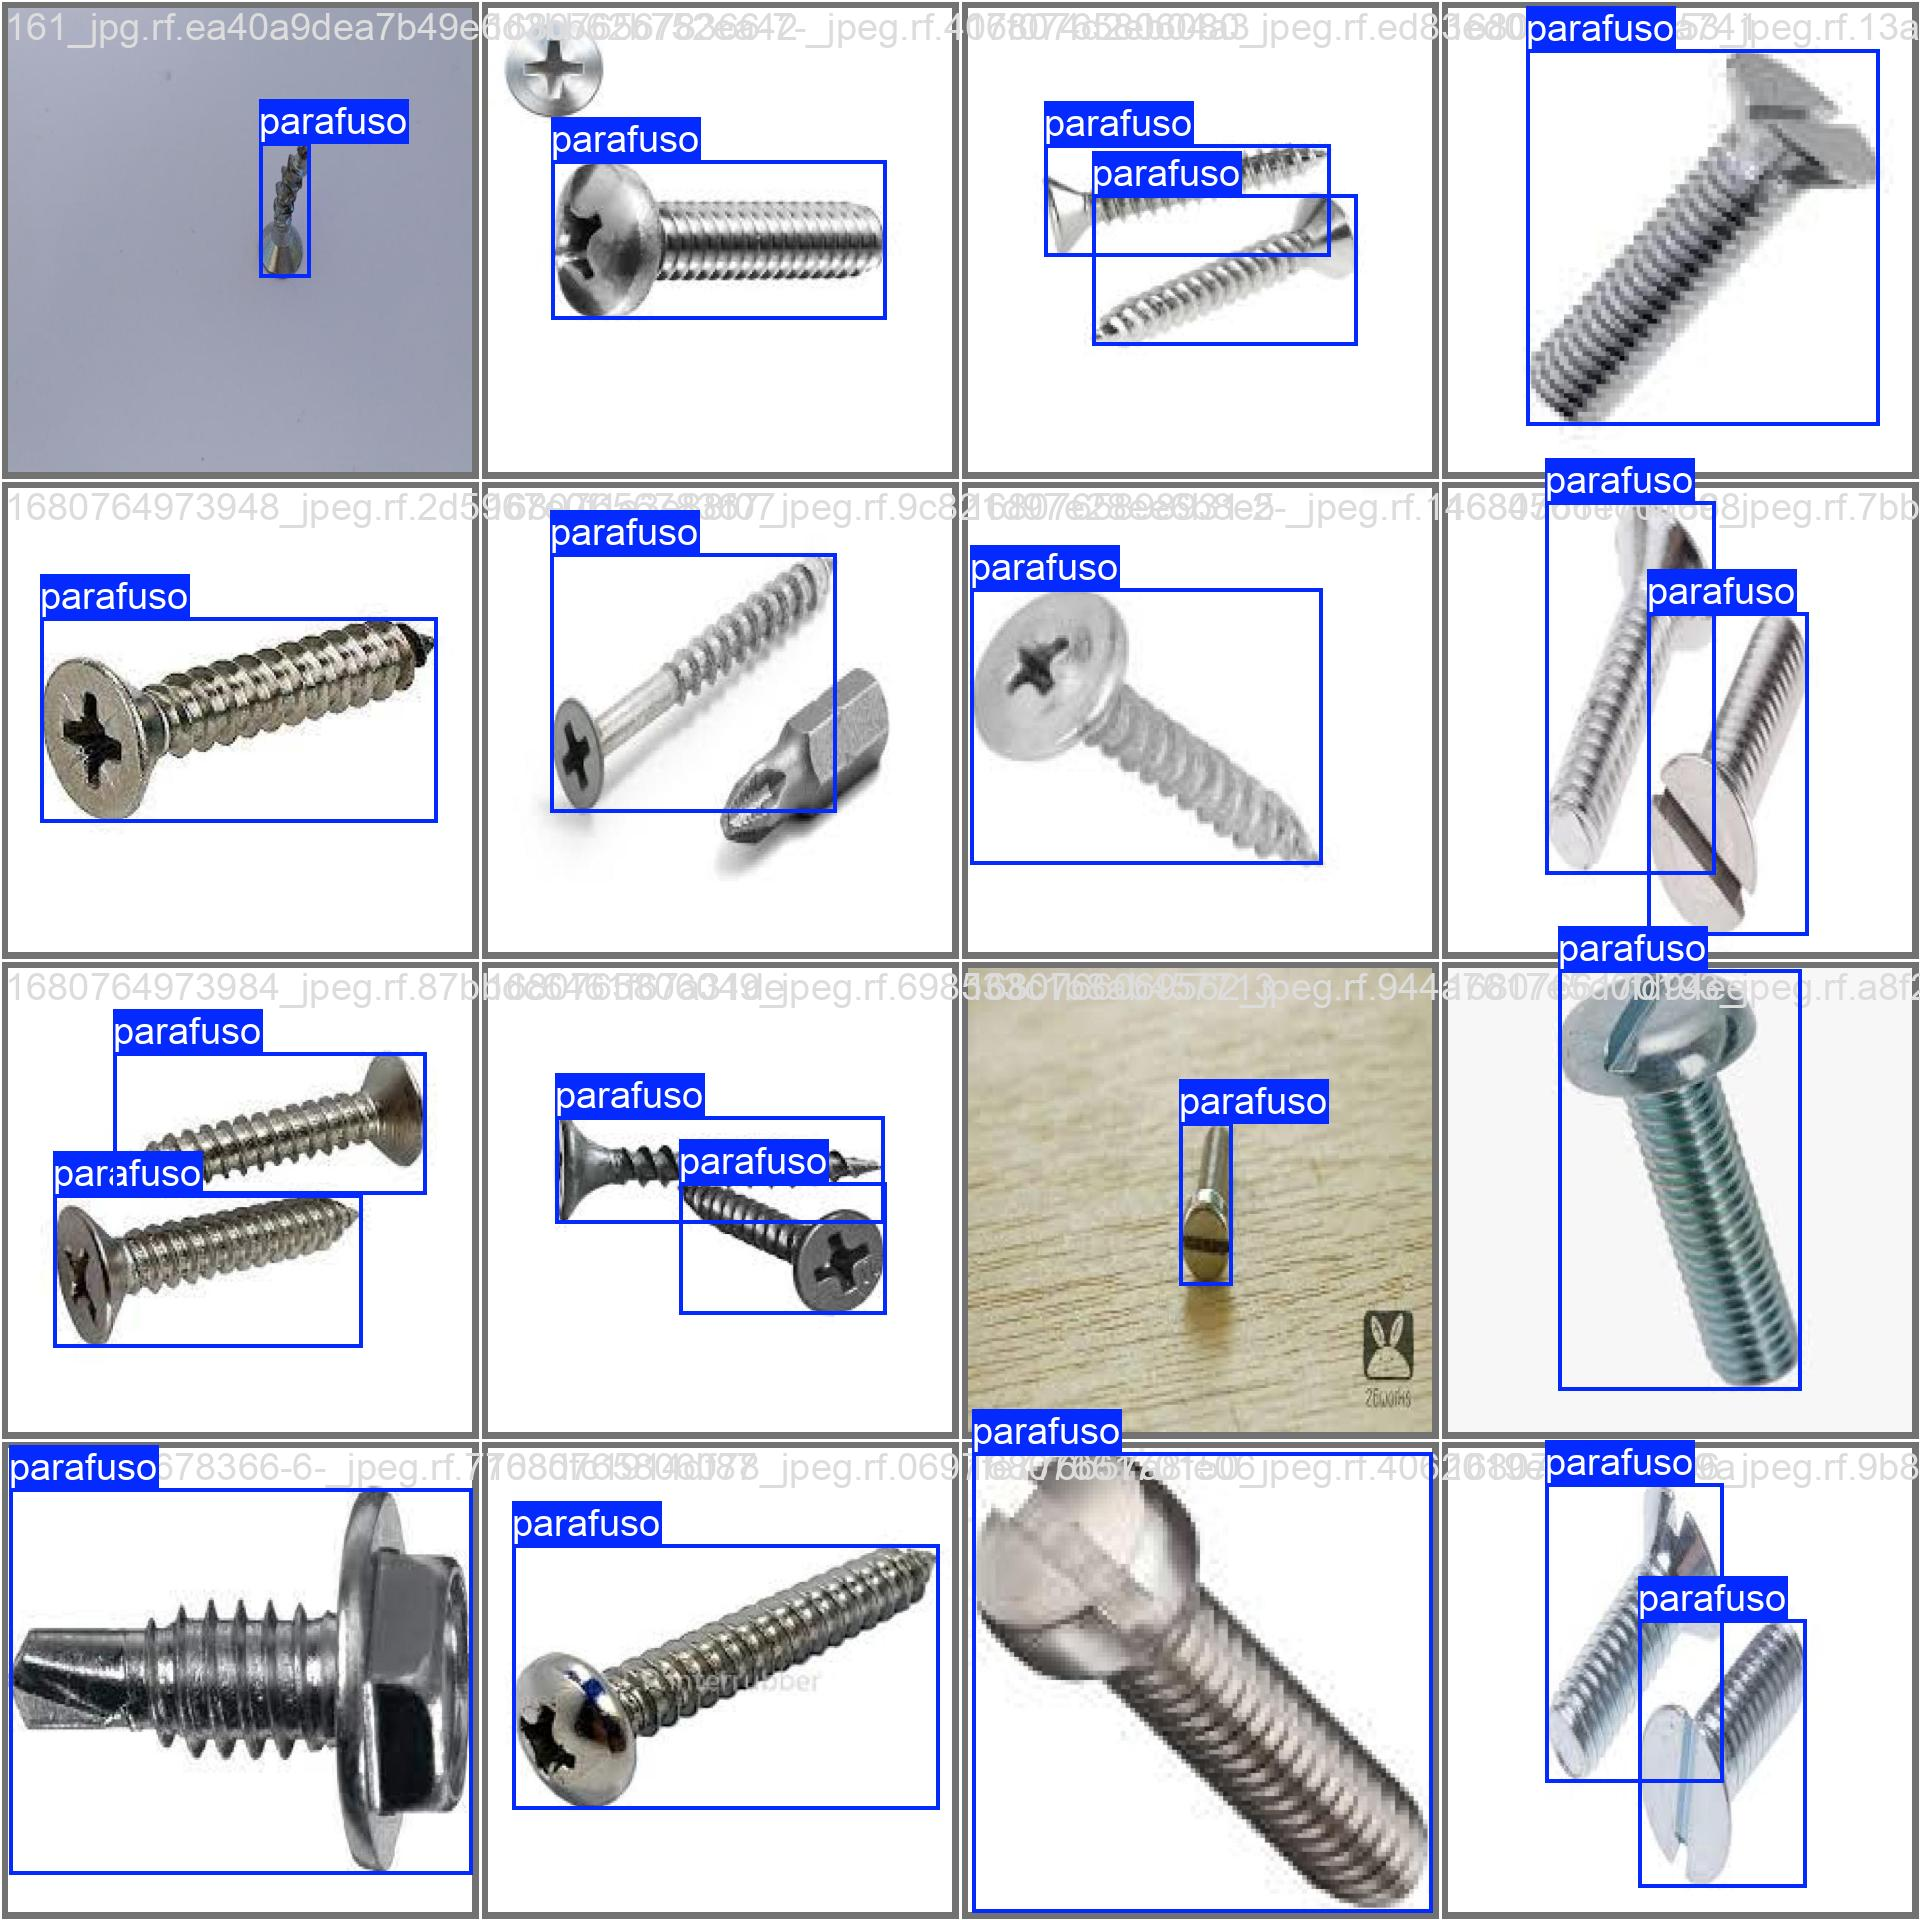
\includegraphics[width=\linewidth]{val_batch1_labels.jpg}
    \caption{Lote de valida\c{c}\~ao 1 -- r\'otulos reais}
  \end{subfigure}
  \caption{Lotes de valida\c{c}\~ao com \emph{bounding boxes} anotadas pelo dataset.}
  \label{fig:val-batch}
\end{figure}

\subsection{Resultados Pr\'aticos -- Testes com Novas Imagens}

O modelo YOLOv11 foi testado com novas imagens n\~ao vistas durante o treinamento.
A Figura~\ref{fig:yolo-resultados} mostra a detec\c{c}\~ao em tr\^es cen\'arios
distintos, com as \emph{bounding boxes} e pontuac\~oes de confian\c{c}a exibidas
sobre cada parafuso detectado.

\begin{figure}[H]
  \centering
  \begin{subfigure}[t]{0.31\textwidth}
    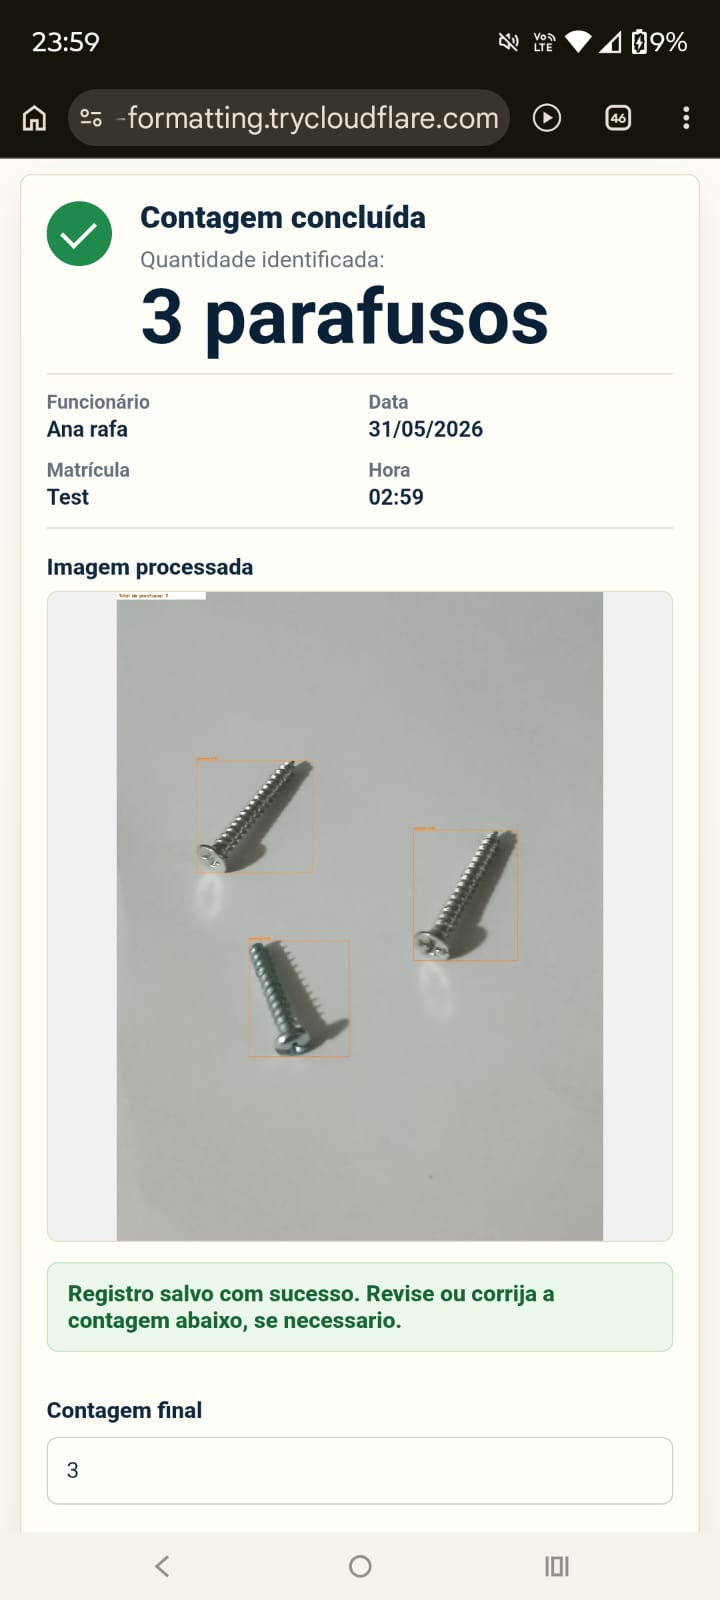
\includegraphics[width=\linewidth]{yolo1.jpeg}
    \caption{Resultado YOLO -- imagem 1}
  \end{subfigure}\hfill
  \begin{subfigure}[t]{0.31\textwidth}
    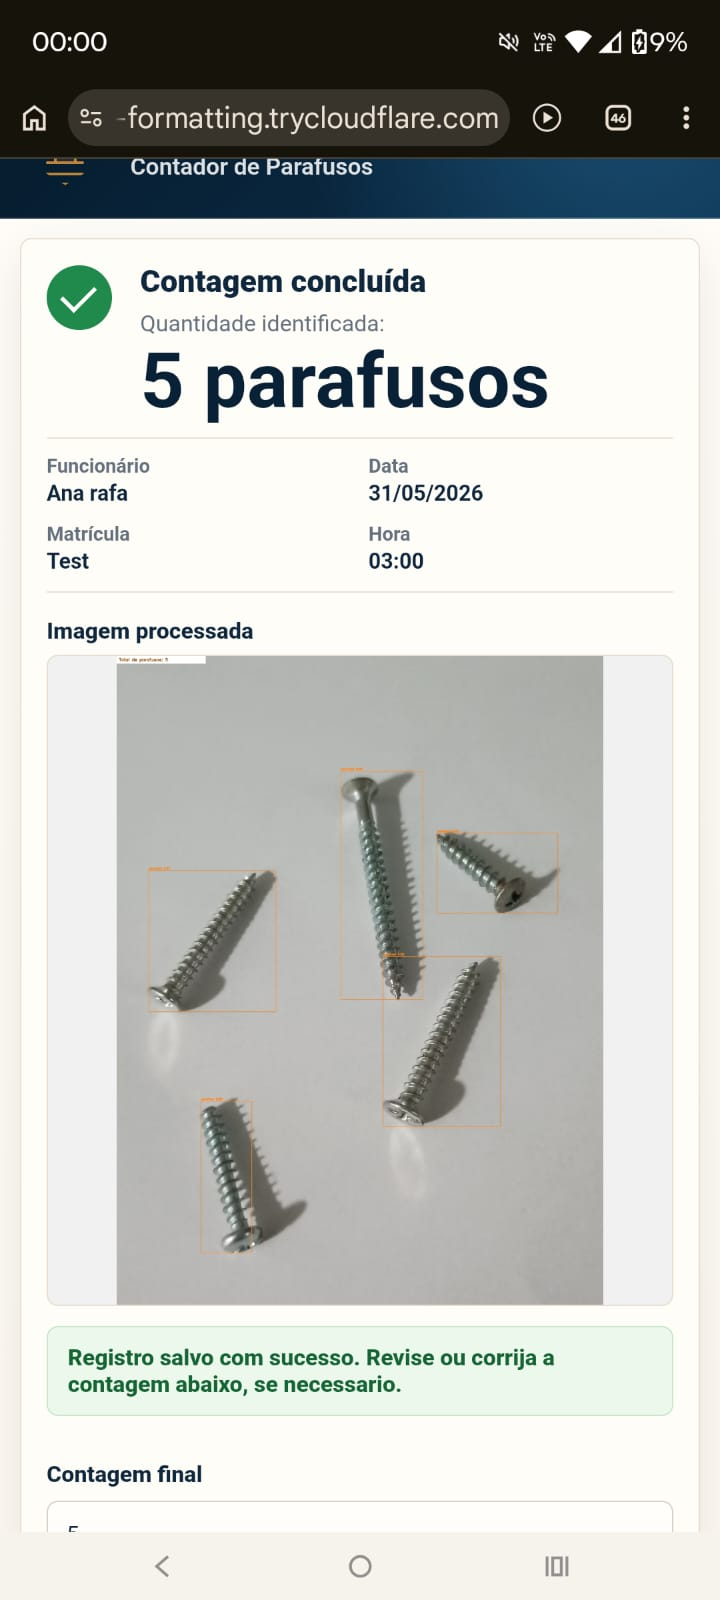
\includegraphics[width=\linewidth]{yolo2.jpeg}
    \caption{Resultado YOLO -- imagem 2}
  \end{subfigure}\hfill
  \begin{subfigure}[t]{0.31\textwidth}
    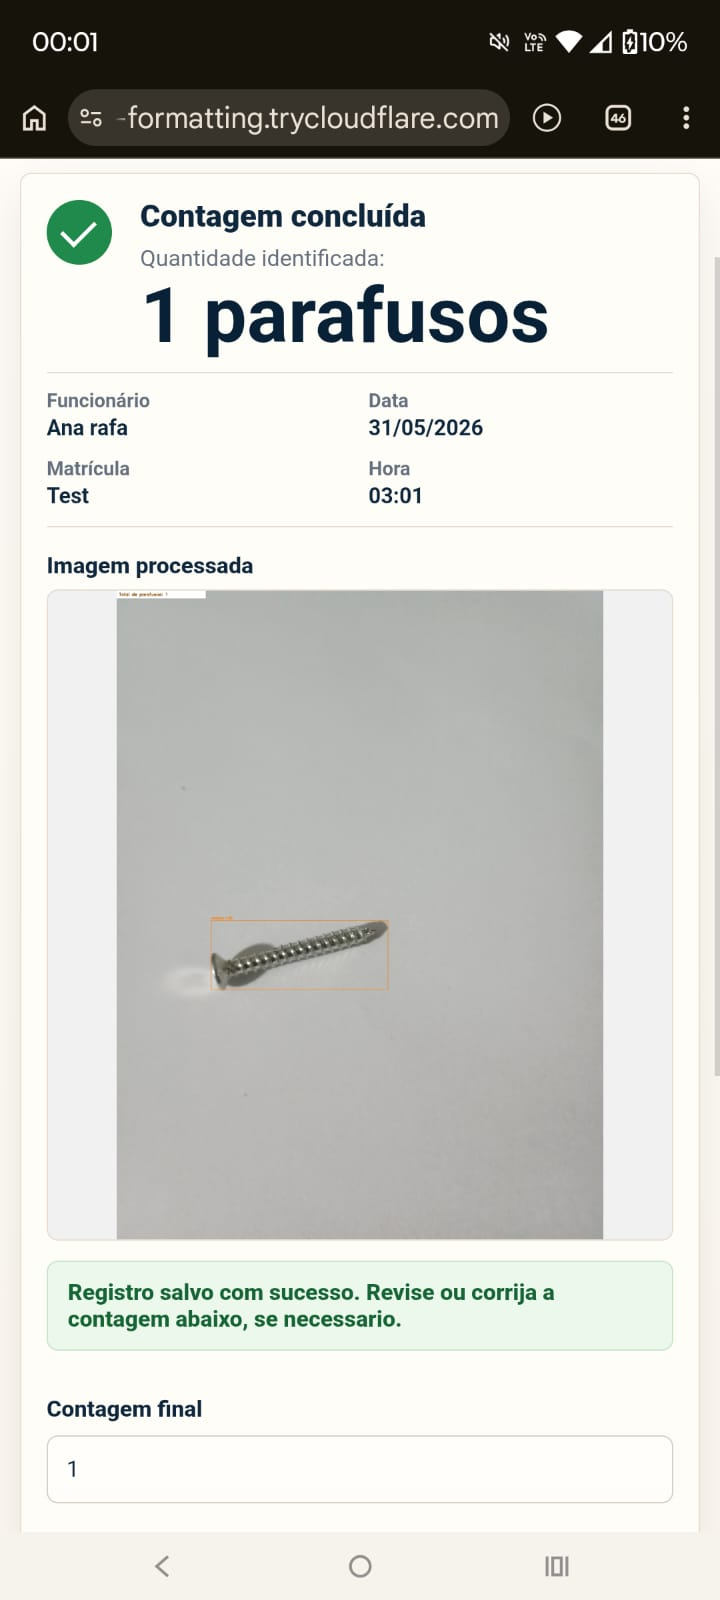
\includegraphics[width=\linewidth]{yolo3.jpeg}
    \caption{Resultado YOLO -- imagem 3}
  \end{subfigure}
  \caption{Resultados pr\'aticos do YOLOv11 em novas imagens: cada caixa exibe o
           r\'otulo \texttt{parafuso} e a confian\c{c}a da detec\c{c}\~ao.}
  \label{fig:yolo-resultados}
\end{figure}

%% ============================================================
\section{Aplica\c{c}\~ao Web Compartilhada}
\label{sec:web}

Ambas as solu\c{c}\~oes compartilham a mesma arquitetura de aplica\c{c}\~ao web
baseada em \textbf{FastAPI} + \textbf{Jinja2} + \textbf{SQLite}.

\subsection{Por que FastAPI?}

\begin{itemize}[leftmargin=*]
  \item Alta performance (Starlette/Uvicorn, ass\'incrono por padr\~ao).
  \item Valida\c{c}\~ao autom\'atica de dados com Pydantic.
  \item Suporte nativo a upload de arquivos (\texttt{UploadFile}).
  \item Gera\c{c}\~ao autom\'atica de documenta\c{c}\~ao interativa em \texttt{/docs}.
\end{itemize}

\subsection{Fluxo de uma requisi\c{c}\~ao}

\begin{enumerate}[leftmargin=*, label=\arabic*.]
  \item Operador acessa a interface via smartphone (Wi-Fi local).
  \item Faz login: nome, matr\'icula e setor s\~ao salvos em \emph{cookies} (12\,h).
  \item Envia a foto pelo formul\'ario HTML responsivo.
  \item \texttt{POST /predict} recebe o arquivo, salva em disco, chama o contador
        (vis\~ao cl\'assica ou YOLO) e persiste no banco de dados.
  \item A p\'agina de resultado exibe imagem anotada e total.
  \item Operador pode corrigir manualmente a contagem.
\end{enumerate}

\subsection{Rotas Principais}

\begin{table}[H]
  \centering
  \caption{Rotas da API}
  \label{tab:rotas}
  \begin{tabular}{lll}
    \toprule
    \textbf{M\'etodo} & \textbf{Rota} & \textbf{Descri\c{c}\~ao} \\
    \midrule
    GET  & \texttt{/}                      & P\'agina inicial / envio de foto \\
    POST & \texttt{/login}                 & Autentica\c{c}\~ao por cookie \\
    POST & \texttt{/logout}                & Encerramento de sess\~ao \\
    POST & \texttt{/predict}               & Infer\^encia e registro \\
    GET  & \texttt{/dashboard}             & Hist\'orico de contagens \\
    POST & \texttt{/record/\{id\}/correct} & Corre\c{c}\~ao manual \\
    POST & \texttt{/finalizar-dia}         & Gera CSV + PDF do fechamento do dia \\
    GET  & \texttt{/export/csv}            & Exporta\c{c}\~ao completa em CSV \\
    GET  & \texttt{/export/csv/today}      & Exporta\c{c}\~ao do dia \\
    GET  & \texttt{/export/pdf/today}      & Exporta\c{c}\~ao em PDF (Solu\c{c}\~ao 1) \\
    GET  & \texttt{/health}               & Status do sistema \\
    \bottomrule
  \end{tabular}
\end{table}

\subsection{Banco de Dados -- Modelo ORM}

O sistema utiliza \textbf{SQLite} via \textbf{SQLAlchemy ORM}. A migra\c{c}\~ao
futura para PostgreSQL requer apenas alterar \texttt{DATABASE\_URL} em
\texttt{config.py}.

\begin{lstlisting}[caption={Modelo de dados compartilhado (\texttt{app/models.py})}]
class Contagem(Base):
    __tablename__ = "contagens"
    id               = Column(Integer,     primary_key=True)
    funcionario_nome = Column(String(160), nullable=False)
    funcionario_id   = Column(String(80),  nullable=True)
    setor            = Column(String(120), nullable=True)
    pedido           = Column(String(120), nullable=True)
    data_hora        = Column(DateTime,    server_default=func.now())
    total_parafusos  = Column(Integer,     nullable=False)
    total_corrigido  = Column(Integer,     nullable=True)  # correcao manual
    confianca_media  = Column(Float,       nullable=False)
    imagem_original  = Column(Text,        nullable=False)
    imagem_processada = Column(Text,       nullable=False)
    status           = Column(String(40),  nullable=True)  # confirmada/corrigida
    observacao       = Column(Text,        nullable=True)
\end{lstlisting}

\subsection{Funcionalidades Exclusivas da Solu\c{c}\~ao 1 (Web)}

A Solu\c{c}\~ao 1 implementa funcionalidades adicionais no backend:

\begin{itemize}[leftmargin=*]
  \item \textbf{Relat\'orio PDF autom\'atico}: gerado com \texttt{Pillow} (\texttt{build\_pdf\_report}),
        com cabe\c{c}alho corporativo, tabela paginada de registros e cards de resumo.
  \item \textbf{Fechamento di\'ario}: rota \texttt{/finalizar-dia} consolida todos os
        registros do dia em CSV + PDF + JSON e salva em \texttt{outputs/fechamentos/}.
  \item \textbf{Agrupamento por dia} no dashboard (\texttt{group\_records\_by\_day}).
\end{itemize}

\subsection{Conex\~ao via Smartphone}

A fun\c{c}\~ao \texttt{get\_local\_ip()} detecta automaticamente o IP da m\'aquina
e exibe na tela inicial para facilitar o acesso via Wi-Fi:

\begin{lstlisting}[caption={Detec\c{c}\~ao autom\'atica de IP local}]
def get_local_ip() -> str:
    try:
        sock = socket.socket(socket.AF_INET, socket.SOCK_DGRAM)
        sock.connect(("8.8.8.8", 80))   # Nao envia dados; usa rota padrao
        ip = sock.getsockname()[0]
        sock.close()
        return ip
    except Exception:
        return "127.0.0.1"
\end{lstlisting}

%% ============================================================
\section{Processo de Design -- UX/UI da Aplica\c{c}\~ao}
\label{sec:uxui}

\subsection{Contexto e Objetivos do Design}

O design da interface foi guiado por tr\^es princ\'ipios fundamentais, diretamente
relacionados ao perfil dos usu\'arios (operadores de \emph{picking} sem treinamento
t\'ecnico e com mãos ocupadas durante o trabalho):

\begin{description}[leftmargin=*, style=nextline]
  \item[Simplicidade radical:] o fluxo completo -- login, foto, resultado -- deve ser
    conclu\'ido em no m\'aximo tr\^es toques na tela. Nenhuma configura\c{c}\~ao
    t\'ecnica \'e exposta ao operador.

  \item[Feedback imediato:] o resultado da contagem \'e exibido em destaque logo ap\'os
    o envio da imagem, com a foto anotada ao lado para inspe\c{c}\~ao visual r\'apida.

  \item[Recupera\c{c}\~ao de erros:] todo registro permite corre\c{c}\~ao manual com
    um campo num\'erico simples, garantindo que nenhum erro do modelo impacte o processo
    de forma irrecuper\'avel.
\end{description}

\subsection{Prot\'otipo de Interface -- UX/UI}

O prot\'otipo foi criado antes da implementa\c{c}\~ao do \emph{backend}, seguindo a
metodologia \emph{design-first}: as telas foram validadas conceitualmente antes do
desenvolvimento, garantindo que a estrutura do c\'odigo suportasse exatamente o fluxo
projetado.

A Figura~\ref{fig:prototipo} apresenta o prot\'otipo de alta fidelidade da aplica\c{c}\~ao,
cobrindo as telas principais: login do operador, envio de imagem, resultado da contagem,
hist\'orico do dia e dashboard de gest\~ao.

\begin{figure}[H]
  \centering
  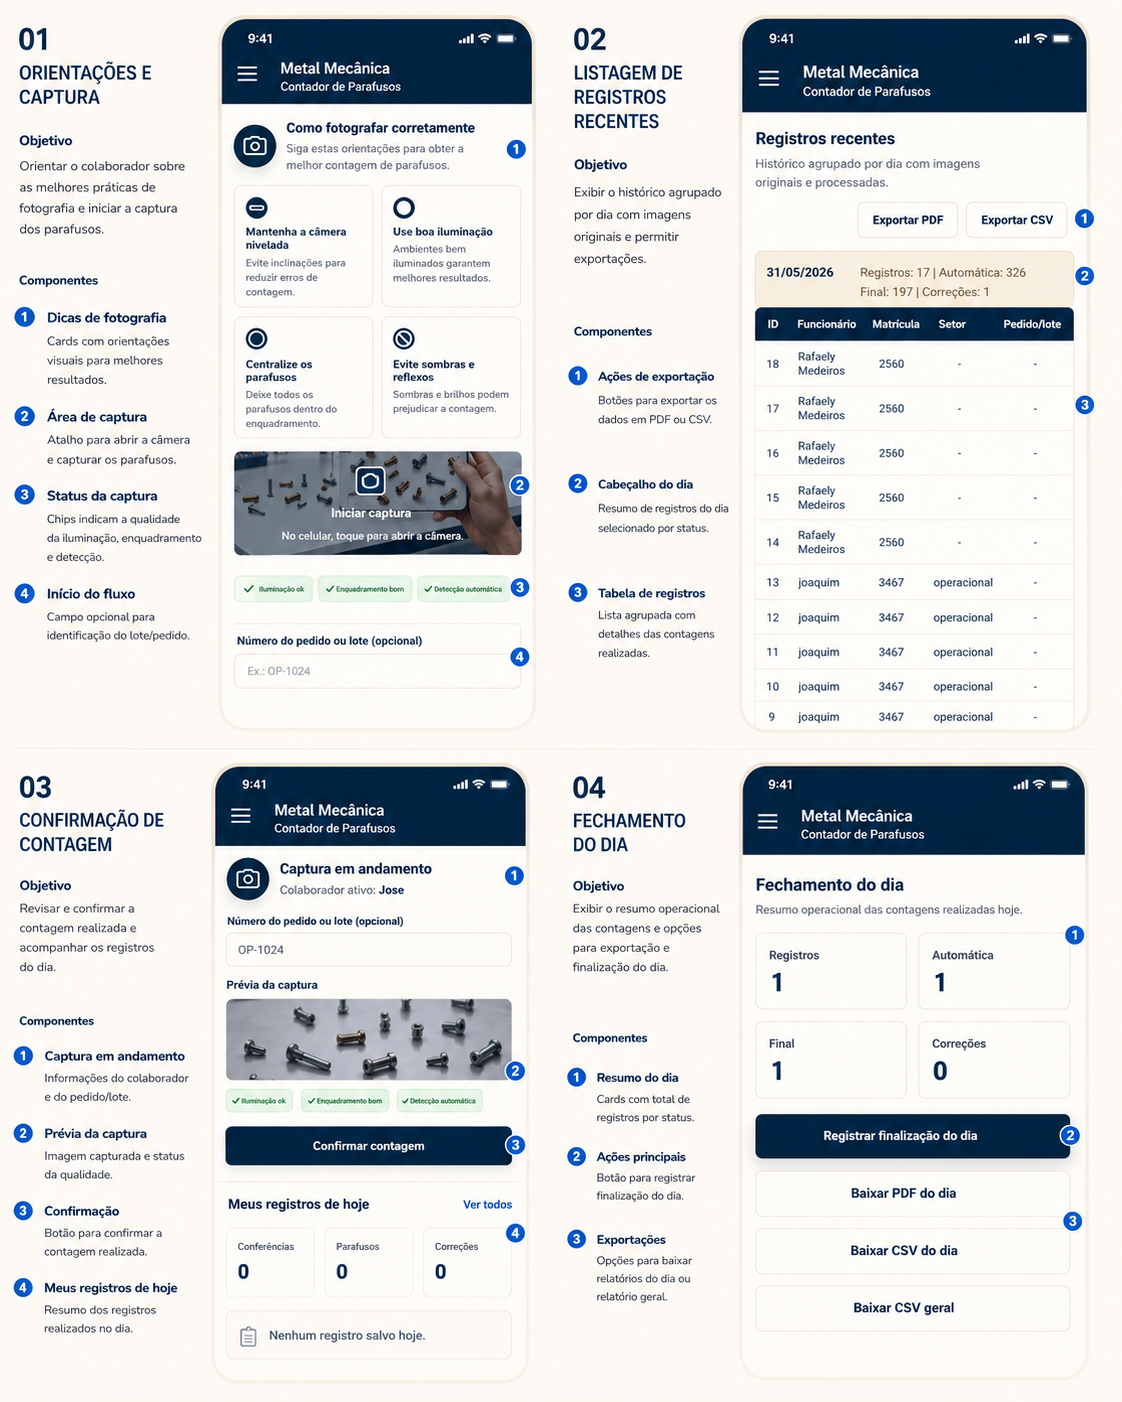
\includegraphics[width=\linewidth]{prototipo-designer-ux-ui_app_contagem_parafusos.png}
  \caption{Prot\'otipo UX/UI da aplica\c{c}\~ao de contagem de parafusos. Da esquerda
           para a direita: tela de login, tela de captura/envio de foto, tela de resultado
           com imagem anotada e contador em destaque, hist\'orico do operador e
           dashboard de gest\~ao.}
  \label{fig:prototipo}
\end{figure}

\subsection{Decis\~oes de Design Justificadas}

\begin{table}[H]
  \centering
  \caption{Principais decis\~oes de UX/UI e suas justificativas}
  \label{tab:ux}
  \renewcommand{\arraystretch}{1.2}
  \begin{tabular}{p{4.2cm}p{4.2cm}p{4.2cm}}
    \toprule
    \textbf{Decis\~ao} & \textbf{Alternativa descartada} & \textbf{Justificativa} \\
    \midrule
    Contador central em fonte grande
      & Tabela com detalhes t\'ecnicos
      & Operador precisa confirmar o n\'umero rapidamente, sem ler \\
    Login por nome + matr\'icula
      & Senha alfanum\'erica
      & F\'acil de digitar com luvas; rastreabilidade sem senha \\
    Imagem anotada exibida imediatamente
      & S\'o o n\'umero
      & Permite inspe\c{c}\~ao visual antes de confirmar \\
    Bot\~ao de corre\c{c}\~ao sempre vis\'ivel
      & Corre\c{c}\~ao apenas no dashboard
      & Erro detectado no momento certo, sem voltar telas \\
    Acesso via Wi-Fi + navegador
      & Aplicativo nativo instalado
      & Sem instala\c{c}\~ao, sem atualiza\c{c}\~oes manuais \\
    Dashboard com agrupamento por dia
      & Lista plana cronol\'ogica
      & Facilita o fechamento di\'ario e auditoria por turno \\
    \bottomrule
  \end{tabular}
\end{table}

\subsection{Fluxo de Navega\c{c}\~ao}

\begin{center}
\fbox{
\begin{minipage}{0.88\textwidth}
\centering
\textbf{Login} (nome + matr\'icula + setor)\\
$\downarrow$\\
\textbf{Tela principal} -- enviar foto do pedido\\
$\downarrow$\\
\textbf{Resultado} -- contador + imagem anotada + campo de corre\c{c}\~ao\\
$\downarrow$ \quad\quad $\swarrow$ (se correto)\\
\textbf{Dashboard} -- hist\'orico agrupado por dia + fechamento\\
$\downarrow$\\
\textbf{Exporta\c{c}\~ao} -- CSV ou PDF corporativo
\end{minipage}
}
\end{center}

\subsection{Responsividade e Compatibilidade Mobile}

A interface foi projetada para funcionar em \textbf{qualquer navegador moderno}, sem
instala\c{c}\~ao de aplicativo. Os pontos-chave de responsividade s\~ao:

\begin{itemize}[leftmargin=*]
  \item Layout em coluna \'unica em telas estreitas (\emph{smartphones}).
  \item Bot\~oes com \'area de toque m\'inima de 48$\times$48\,px (diretrizes WCAG).
  \item Campo de upload de foto ativando diretamente a c\^amera do dispositivo
        (\texttt{accept="image/*"} + \texttt{capture="environment"}).
  \item IP do servidor exibido automaticamente na tela inicial para facilitar
        a conex\~ao dos operadores na rede Wi-Fi.
\end{itemize}

%% ============================================================
\section{An\'alise Comparativa das Solu\c{c}\~oes}
\label{sec:comparativo}

\subsection{Compara\c{c}\~ao T\'ecnica}

\begin{table}[H]
  \centering
  \caption{Compara\c{c}\~ao direta entre as duas solu\c{c}\~oes}
  \label{tab:comp}
  \renewcommand{\arraystretch}{1.25}
  \begin{tabular}{p{4.2cm}p{4.5cm}p{4.5cm}}
    \toprule
    \textbf{Aspecto} & \textbf{Solu\c{c}\~ao 1 (OpenCV)} &
    \textbf{Solu\c{c}\~ao 2 (YOLOv11)} \\
    \midrule
    Dados necess\'arios
      & Zero (nenhum label)
      & Dataset anotado (Roboflow Screw v4) \\
    Treinamento
      & Nenhum
      & $\sim$\,2\,h GPU (100 \'epocas) \\
    Tamanho do modelo
      & $\sim$\,0\,MB (c\'odigo puro)
      & $\sim$\,20\,MB (\texttt{yolo11s}) \\
    Velocidade (CPU)
      & $<$\,200\,ms por imagem
      & $\sim$\,300--800\,ms por imagem \\
    Precis\~ao geral
      & Moderada (sens\'ivel ao cen\'ario)
      & Alta (robusta a varia\c{c}\~oes) \\
    Parafusos sobrepostos
      & Watershed / DBSCAN (parcial)
      & NMS por IoU (muito melhor) \\
    Varia\c{c}\~ao de fundo
      & Depend\^encia moderada/alta
      & Praticamente independente \\
    Interpretabilidade
      & Alta (cada etapa visu\'avel)
      & M\'edia (caixa preta parcial) \\
    Exporta\c{c}\~ao mobile
      & N/A (OpenCV \'e leve o suficiente)
      & TFLite / NCNN / CoreML \\
    Depend\^encias extras
      & OpenCV, scikit-learn
      & PyTorch, Ultralytics \\
    Curva de aprendizado
      & Baixa
      & M\'edia (configura\c{c}\~ao de treino) \\
    Escalabilidade
      & Manual (ajuste de par\^ametros)
      & Alta (basta anotar mais dados) \\
    \bottomrule
  \end{tabular}
\end{table}

\subsection{Cen\'arios Favor\'aveis a Cada Solu\c{c}\~ao}

\begin{table}[H]
  \centering
  \caption{Quando usar cada solu\c{c}\~ao}
  \label{tab:quando}
  \begin{tabular}{p{5.8cm}p{5.8cm}}
    \toprule
    \textbf{Solu\c{c}\~ao 1 -- Vis\~ao Cl\'assica} &
    \textbf{Solu\c{c}\~ao 2 -- YOLOv11} \\
    \midrule
    Implanta\c{c}\~ao imediata (sem GPU)
      & Ambiente de produ\c{c}\~ao exigente \\
    Poucas imagens dispon\'iveis
      & Grande volume de parafusos por foto \\
    Rastreabilidade do pipeline obrigat\'oria
      & Parafusos com sobreposic\~ao frequente \\
    Fundo controlado (branco/neutro)
      & Cen\'arios variados de ilumina\c{c}\~ao \\
    Valida\c{c}\~ao r\'apida da viabilidade
      & Sistema em expans\~ao (novas categorias) \\
    \bottomrule
  \end{tabular}
\end{table}

%% ============================================================
\section{Veredicto: Qual Solu\c{c}\~ao \'e Melhor?}
\label{sec:veredicto}

\begin{tcolorbox}[veredicto={Recomenda\c{c}\~ao T\'ecnica}]

\textbf{Para o contexto do Desafio 1, a Solu\c{c}\~ao 2 (YOLOv11) \'e a mais
recomendada para implanta\c{c}\~ao em produ\c{c}\~ao.}

\medskip
Os motivos principais s\~ao:

\begin{enumerate}[leftmargin=*, label=\arabic*.]
  \item \textbf{Robustez:} o processo de \emph{picking} ocorre em ambientes reais, com
        varia\c{c}\~ao de ilumina\c{c}\~ao, \^angulo e fundo. O YOLOv11 aprende
        invariâncias diretamente dos dados, enquanto a Solu\c{c}\~ao 1 depende de
        ajuste manual de par\^ametros para cada cen\'ario.

  \item \textbf{Precis\~ao em aglomerados:} parafusos sobrepostos s\~ao o principal
        desafio do \emph{picking}. O NMS (\emph{Non-Maximum Suppression}) do YOLO
        lida nativamente com isso; o watershed da Solu\c{c}\~ao 1 tem desempenho
        vari\'avel.

  \item \textbf{Escalabilidade:} quando a empresa ampliar o cat\'alogo (novos tipos
        de parafuso, arruelas, porcas), basta anotar exemplos e fazer
        \emph{fine-tuning}, sem reescrever o pipeline.

  \item \textbf{Mobile-ready:} a Solu\c{c}\~ao 2 inclui scripts de exporta\c{c}\~ao
        para TFLite, NCNN e CoreML, habilitando infer\^encia diretamente no
        smartphone, sem servidor.
\end{enumerate}

\medskip
\textbf{Ressalva:} a Solu\c{c}\~ao 1 tem papel estrat\'egico como
\emph{baseline} interpret\'avel e deve ser mantida para:
\begin{itemize}[leftmargin=*, noitemsep]
  \item Valida\c{c}\~ao imediata em ambientes sem GPU;
  \item Auditoria e depura\c{c}\~ao de casos-limite;
  \item Cen\'arios controlados com fundo neutro onde \'e suficiente.
\end{itemize}

\end{tcolorbox}

%% ============================================================
\section{Crit\'erios de Avalia\c{c}\~ao -- Resposta Direta}

\subsection{1. Organiza\c{c}\~ao e Estrutura\c{c}\~ao do C\'odigo}

As duas solu\c{c}\~oes seguem o princ\'ipio de \emph{separa\c{c}\~ao de
responsabilidades}:

\begin{itemize}[leftmargin=*]
  \item \textbf{Solu\c{c}\~ao 1:} \texttt{screw\_counter.py} (l\'ogica de vis\~ao),
        \texttt{metrics.py} (avalia\c{c}\~ao), \texttt{evaluation.py} (orquestra\c{c}\~ao
        de lote), \texttt{main.py} (API), \texttt{app/models.py} (banco de dados).
  \item \textbf{Solu\c{c}\~ao 2:} \texttt{screw\_counter.py} (infer\^encia YOLO),
        \texttt{scripts/train\_screws\_yolo.py} (treinamento), \texttt{app/main.py}
        (API), \texttt{app/config.py} (configura\c{c}\~ao centralizada).
  \item \textbf{Compartilhado:} mesma estrutura de banco de dados, rotas, templates
        e l\'ogica de cookie.
\end{itemize}

\subsection{2. Criatividade na Proposta}

\begin{itemize}[leftmargin=*]
  \item Desenvolvimento de \textbf{duas solu\c{c}\~oes} com abordagens complementares.
  \item Sistema de \textbf{ensemble} na Solu\c{c}\~ao 1 com at\'e 19 candidatos.
  \item \textbf{Calibra\c{c}\~ao interativa} por foto de um \'unico parafuso.
  \item Interface web responsiva acess\'ivel diretamente pelo smartphone.
  \item Exporta\c{c}\~ao de relat\'orio \textbf{PDF corporativo} com layout profissional.
  \item \textbf{Fechamento di\'ario} autom\'atico em CSV + PDF + JSON.
  \item Suporte a \textbf{exporta\c{c}\~ao do modelo} para TFLite/NCNN/CoreML.
  \item \textbf{Cache de modelo} para resposta em tempo real sem overhead de I/O.
\end{itemize}

\subsection{3. Clareza nos Crit\'erios de Tomada de Decis\~ao}

Cada decis\~ao t\'ecnica foi fundamentada em crit\'erios expl\'icitos:

\begin{description}[leftmargin=*, style=nextline]
  \item[Escolha do YOLOv11 small:] equil\'ibrio entre precis\~ao e velocidade;
    export\'avel para mobile com quantiza\c{c}\~ao INT8.
  \item[6 modos de segmenta\c{c}\~ao:] cada modo foi projetado para uma categoria
    visual espec\'ifica de cena, com crit\'erios de sele\c{c}\~ao baseados em
    estat\'isticas objetivas (brilho, contraste, textura, densidade).
  \item[\texttt{CONF=0.25, IOU=0.45}:] ponto de partida conservador document\'avel
    e ajust\'avel sem recompila\c{c}\~ao.
  \item[SQLite:] elimina depend\^encia de servidor externo; migra\c{c}\~ao a
    PostgreSQL via troca de uma linha em \texttt{config.py}.
  \item[Cookie de sess\~ao:] sem servidor de sess\~oes externo, sistema autocontido.
\end{description}

\subsection{4. Capacidade Anal\'itica}

\begin{itemize}[leftmargin=*]
  \item M\'odulo completo de m\'etricas (\texttt{metrics.py}) com MAE, acur\'acia
        exata, vi\'es m\'edio, supercontagens e subcontagens.
  \item Script de \emph{grid search} de hiperpar\^ametros (\texttt{grid\_search\_parameters})
        com resultado tabelado.
  \item Notebook Jupyter (\texttt{notebooks/analise\_treinamento\_parafusos\_yolo11.ipynb})
        com curvas de perda, mAP por \'epoca, varredura de confian\c{c}a e CSV
        comparativo.
  \item Alerta autom\'atico de qualidade de captura com diagn\'ostico (blur, borda,
        dist\^ancia).
\end{itemize}

\subsection{B\^onus: Solu\c{c}\~ao em Aplica\c{c}\~ao Web}

\checkmark\ Ambas as solu\c{c}\~oes possuem interface web responsiva acess\'ivel
pelo smartphone via navegador (Wi-Fi local), sem instala\c{c}\~ao de aplicativo.

\subsection{B\^onus: Baixo Recurso Computacional}

\checkmark\ A Solu\c{c}\~ao 1 roda em qualquer CPU com OpenCV. \\
\checkmark\ A Solu\c{c}\~ao 2 inclui scripts de exporta\c{c}\~ao para TFLite, NCNN e
CoreML para infer\^encia nativa no smartphone.

%% ============================================================
\section{Instru\c{c}\~oes de Execu\c{c}\~ao}

\subsection{Solu\c{c}\~ao 1 -- Vis\~ao Cl\'assica}

\begin{lstlisting}[language=bash, caption={Iniciar a Solu\c{c}\~ao 1}]
cd solucao_1_visao_classica
pip install -r requirements.txt
uvicorn main:app --reload --host 0.0.0.0 --port 8000
\end{lstlisting}

Acesso no smartphone (mesma rede Wi-Fi):
\begin{verbatim}
http://<IP_DO_SERVIDOR>:8000
\end{verbatim}


Para descobrir o IP do servidor no Windows:

\begin{lstlisting}[caption={Verificar IP local do servidor}]
ipconfig
\end{lstlisting}

Acesso no smartphone por túnel:

\begin{lstlisting}[caption={Criar túnel público para acesso via smartphone}]
winget install --id Cloudflare.cloudflared
cloudflared tunnel --url http://localhost:8000
\end{lstlisting}

Após executar o comando, acessar no smartphone a URL HTTPS gerada pelo terminal:

\begin{verbatim}
https://<URL_GERADA>.trycloudflare.com
\end{verbatim}

\subsection{Solu\c{c}\~ao 2 -- YOLOv11}

\begin{lstlisting}[language=bash, caption={Prepara\c{c}\~ao e execu\c{c}\~ao da Solu\c{c}\~ao 2}]
cd solucao_2_yolo
pip install -r requirements.txt

# Converter dataset (uma vez)
python scripts/convert_segments_to_boxes.py \
  --input  Screw.v4-dataset-screw4.yolov11 \
  --output dataset_detect

# Treinar modelo
python scripts/train_screws_yolo.py \
  --data dataset_detect/data.yaml \
  --model yolo11s.pt --epochs 100 --imgsz 960

# Validar modelo (gera P, R, mAP50, mAP50-95 em validation_report.txt)
python scripts/validate_screws_yolo.py \
  --data dataset_detect/data.yaml \
  --model runs_screws/yolo11_screws-2/weights/best.pt

# Iniciar aplicacao web
uvicorn app.main:app --reload --host 0.0.0.0 --port 8000
\end{lstlisting}

Para descobrir o IP do servidor no Windows:

\begin{lstlisting}[caption={Verificar IP local do servidor}]
ipconfig
\end{lstlisting}

Acesso no smartphone por túnel:

\begin{lstlisting}[caption={Criar túnel público para acesso via smartphone}]
winget install --id Cloudflare.cloudflared
cloudflared tunnel --url http://localhost:8000
\end{lstlisting}

Após executar o comando, acessar no smartphone a URL HTTPS gerada pelo terminal:

\begin{verbatim}
https://<URL_GERADA>.trycloudflare.com
\end{verbatim}

%% ============================================================
\section{Conclus\~ao}

Este trabalho apresentou duas solu\c{c}\~oes completas e funcionais para o problema
de contagem autom\'atica de parafusos no processo de picking industrial:

\begin{enumerate}[leftmargin=*, label=\arabic*.]
  \item A \textbf{Solu\c{c}\~ao 1 (Vis\~ao Cl\'assica)} demonstra que \'e poss\'ivel
        obter resultados aceit\'aveis sem dados anotados, usando um pipeline
        interpret\'avel com ensemble de modos e detectores. \'E a escolha ideal
        para valida\c{c}\~ao r\'apida e ambientes controlados.

  \item A \textbf{Solu\c{c}\~ao 2 (YOLOv11)} \'e a abordagem recomendada para
        produ\c{c}\~ao: mais robusta, precisa, escal\'avel e com suporte nativo
        \`a plataforma mobile.
\end{enumerate}

Ambas compartilham a mesma aplica\c{c}\~ao web FastAPI, com hist\'orico de
contagens, corre\c{c}\~ao manual, exporta\c{c}\~ao CSV/PDF e acesso direto pelo
smartphone, atendendo tanto aos requisitos obrigat\'orios quanto aos b\^onus
do Desafio 1.

\medskip
Por fim, registrou-se o \textbf{SAM3} (modelo fundacional de segmenta\c{c}\~ao) como
\textbf{caminho de evolu\c{c}\~ao escal\'avel} (Se\c{c}\~ao~\ref{sec:sam3}): inaplic\'avel
ao cen\'ario atual por exigir GPU dedicada -- incompat\'ivel com os smartphones de baixo
custo da empresa -- mas uma op\c{c}\~ao poderosa caso a empresa venha a investir em um
servidor central com GPU no futuro. O modelo YOLOv11 entregue, com \textbf{mAP50 de
98,8\%} e precision/recall acima de 97\% (Se\c{c}\~ao~\ref{sec:metricas-yolo}), atende
plenamente \`a necessidade presente, mantendo o caminho aberto para essa evolu\c{c}\~ao.

%% ============================================================
\appendix
\section{Estrutura de Arquivos}

\begin{verbatim}
desafio-1/
  solucao_1_visao_classica/
    screw_counter.py     # Pipeline classico (6 modos, 3 detectores, ensemble)
    metrics.py           # MAE, acuracia exata, vies medio
    evaluation.py        # Avaliacao em lote + grid search
    main.py              # API FastAPI (10 rotas, PDF, fechamento)
    contador_parafusos_web.py  # Interface para o backend web
    app/
      config.py / database.py / models.py
      static/ / templates/
  solucao_2_yolo/
    screw_counter.py     # Inferencia YOLOv11 com cache de modelo
    app/
      main.py / config.py / database.py / models.py
      services/screw_counter.py
      static/ / templates/
    scripts/
      train_screws_yolo.py
      validate_screws_yolo.py
      convert_segments_to_boxes.py
      export_tflite.py / export_ncnn.py / export_coreml.py
    notebooks/
      analise_treinamento_parafusos_yolo11.ipynb
\end{verbatim}

\section{Depend\^encias Principais}

\begin{table}[H]
  \centering
  \caption{Bibliotecas Python utilizadas}
  \begin{tabular}{llll}
    \toprule
    \textbf{Biblioteca} & \textbf{Solu\c{c}\~ao 1} & \textbf{Solu\c{c}\~ao 2} &
    \textbf{Finalidade} \\
    \midrule
    opencv-python & \checkmark & \checkmark & Vis\~ao computacional \\
    fastapi       & \checkmark & \checkmark & API HTTP \\
    uvicorn       & \checkmark & \checkmark & Servidor ASGI \\
    sqlalchemy    & \checkmark & \checkmark & ORM SQLite \\
    jinja2        & \checkmark & \checkmark & Templates HTML \\
    numpy         & \checkmark & \checkmark & Opera\c{c}\~oes num\'ericas \\
    scikit-learn  & \checkmark &            & DBSCAN (clustering) \\
    pillow        & \checkmark &            & Gera\c{c}\~ao de PDF \\
    ultralytics   &            & \checkmark & YOLOv11 \\
    torch         &            & \checkmark & Backend deep learning \\
    pyyaml        &            & \checkmark & Leitura de YAML \\
    \bottomrule
  \end{tabular}
\end{table}

\end{document}
